\documentclass{article}
\usepackage[utf8]{inputenc}
\usepackage[spanish]{babel}
\usepackage{amsmath}
\usepackage{amssymb}
\usepackage{amsfonts}
\usepackage{hyperref}
\usepackage{textcomp}
\usepackage{graphicx}
\usepackage{pgfplots}
\hypersetup{
    colorlinks=true,
    linkcolor=black,
    citecolor=green,
    filecolor=magenta,      
    urlcolor=cyan,
}

\title{Estadística 1}
\author{Jorge Miguel Alvarado Reyes}
\date{16 Agosto 2023}

\begin{document}

\begin{titlepage}
    \begin{center}
        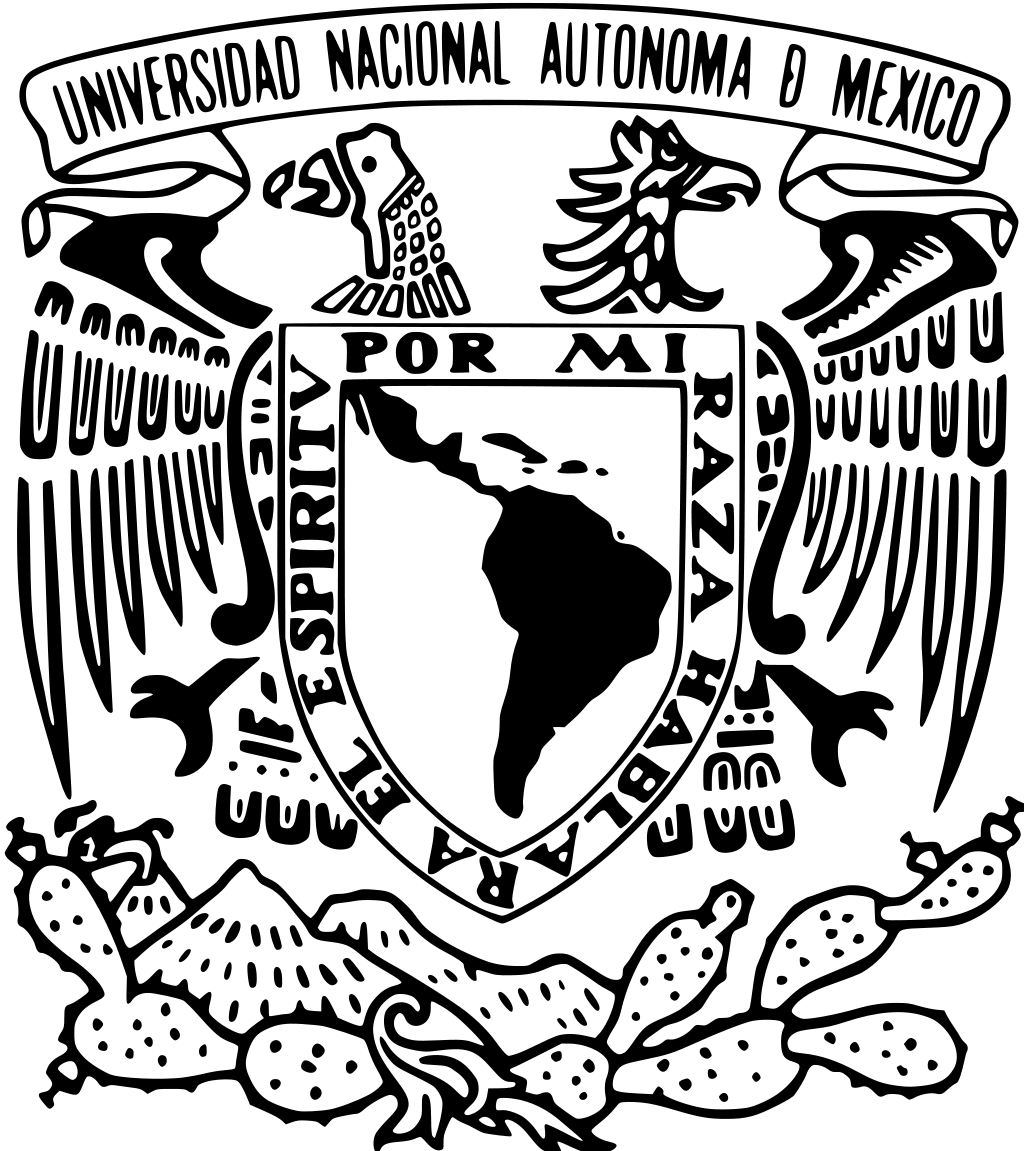
\includegraphics[width=0.2\textwidth]{unam.png}
        \vspace*{.5cm}

        \LARGE
        \textbf{Universidad Nacional Autónoma de México}

        \vspace{0.5cm}
        \LARGE
        Facultad de Estudios Superiores Acatlán

        \vspace{2cm}

        \textbf{Apuntes} \\
        Estadística

        \vfill

        \vspace{1cm}

        \textbf{\large Autor:} \\
        Jorge Miguel Alvarado Reyes \\
        \vspace{.5cm}
        \normalsize \today

    \end{center}
\end{titlepage}
\newpage

\tableofcontents

\newpage

\section{16 de agosto 2023} %Medidas de Tendencia Central

Las medidas de tendencia central son valores de un conjunto de datos que se encuentran en el centro de los datos ordenados.

\subsection{Medidas de Tendencia Central} %media

\subsubsection{Media}

\noindent Existen dos tipos de media: la aritmética y la ponderada.

\noindent La \textbf{media aritmética} se calcula sumando todos los valores y dividiendo por la cantidad de valores:

\[
    \text{Media}(x) = \frac{\sum_{i=1}^{n} x_i}{n} = \frac{1}{n} \cdot \sum_{i=1}^{n}x_i
\]

\textbf{Propiedades}:
\begin{enumerate}
    \item $Media(cx) = c \cdot Media(x)$
    \item $Media(x+c) = Media(x) + c$
\end{enumerate}

\textbf{Ejemplo 4}:

Mostrar que $Media(x+c) = Media(x) + c$.

\textbf{Demostración}:
\[
    \begin{aligned}
        Media(x+c) & = \frac{x_1+c + \ldots + x_n+c}{n}         \\
                   & = \frac{x_1 + \ldots + x_n + n \cdot c}{n} \\
                   & = \frac{x_1 + \ldots + x_n}{n} + c         \\
                   & = Media(x) + c
    \end{aligned}
\]

\textbf{Ejemplo 5}:

Mostrar que $Media(cx) = c \cdot \text{Media}(x)$.

La \textbf{media ponderada} se define como:
\[
    \overline{x} = \frac{\sum_{i=1}^{n} w_i \cdot x_i}{\sum_{i=1}^{n} w_i}
\]

\subsubsection{Mediana}

\noindent La mediana es el valor central que divide a un conjunto de datos ordenados en dos partes iguales. Si $n$ es par, se calcula como:
\[
    Mediana(x) = \frac{x(\frac{n}{2}) + x(\frac{n}{2} + 1)}{2}
\]

% - Estilos -

\subsubsection{Moda}

\noindent Es el valor que mas se repite en un conjunto  de observaciones. \\
\textbf{Ejemplo 6}:

\begin{enumerate}
    \item $[1,2,3,4,5]$ Aqui no existe moda
    \item $[3,4,4,5,5,6]$ Moda = 4.5
    \item $[3,3,4,5,6,6]$ Moda = 3 y 6
    \item $[2,7,7,7,9]$ Moda = 7
\end{enumerate}

\subsection{Media para una serie de frecuencias}

Si $f_1, ... , f_n$ son las frecuencias de la variable $x$. Entonces.
\[
    Mediana(x) = \frac{\sum^{n}_{i=1}f_i \cdot x_i}{\sum^{n}_{i=1}f_i}
\]


\textbf{Ejemplo 7}: \\
Calcula la media para los siguientes valores
\[
    \begin{tabular}{|c|c|}
        \hline
        $x$ & $f_i$ \\
        \hline
        2   & 4     \\
        5   & 1     \\
        6   & 3     \\
        8   & 4     \\
        \hline
    \end{tabular}
\]

\[
    Mediana(x) = \frac{(2\cdot4) + (5\cdot1) + (6\cdot3) + (8\cdot4)}{4+1+3+4} = \frac{8+5+18+32}{12} = \frac{63}{12}
\]

\subsection{Media para datos agrupados}

Sean $f_1, ... , f_n$ las frecuencias de la varible $x$ y $c_1, ... , c_n$ las marcas de clase, entonces: (Marca de clase es un representante)

\[
    Media(x) = \frac{\sum^{n}_{i=1}f_i \cdot c_i}{\sum^{n}_{i=1}f_i}
\]

\textbf{Ejemplo 8}: \\
Calcula la edad promedio para el siguiente conjunto de datos
\[
    \begin{tabular}{|c|c|}
        \hline
        Adulto                    & 25 \\
        \hline
        Adulto de la tercera edad & 10 \\
        \hline
    \end{tabular}
\]

Adulto, edad = [20,65], $c_1 = 43$ \\
Adulto tercera edad, edad = [65,100], $c_1 = 83$\\

25 veces 43 y 10 veces 83

\[
    Mediana(x) = L_{i} t(\frac{\frac{n}{2} - 3 \sum f_i}{f_{mediana}}) \cdot c \\ \\
\]

\noindent $L_i$ = limite inferior de la clase que contiene la mediana\\
$n$ = frecuencia total \\
$\sum f_i$ = suma de las frecuencias menores a la mediana\\
$f_{mediana}$ = Frecuencia de la clase que contiene la mediana\\
$c$ = longitud del intervalo que contiene la mediana \\

\newpage

\section{18 Agosto 2023}

Sitio del curso: https://piazza.com/unam.mx/other/ei20241 \\
codigo de acceso: 150621

\subsection{Breve introduccion a latex}

LaTeX es una herramienta para crear documentos de una gran
calidad tipográfica, en donde los usuarios se ocupan en mayor
medida del contenido del texto en lugar del formato.

\subsubsection{Principales clases de documentos}

\[
    \begin{tabular}{|c|c|}
        \hline
        Clase   & Proposito                                      \\
        \hline
        article & Articulos de revista                           \\
        report  & Textos largos como tesis o reportes            \\
        book    & Libros o documentos con una estructura similar \\
        lette   & cartas                                         \\
        \hline
    \end{tabular}
\]

\subsubsection{Paquetes}

\[
    \begin{tabular}{|c|c|}
        \hline
        Nombre                    & Función                                  \\
        \hline
        amsmath, amssymb, amsfont & Permiten el uso de símbolos matemáticos. \\
        babel                     & Escribir en diversos idiomas.            \\
        inputec                   & Codificacion de entradas.                \\
        \hline
    \end{tabular}
\]

\subsubsection{Estructura de un documento}

\begin{verbatim}
    \documentclass[11pt, a4paper]{report}
    \usepackage[utf8]{inputec}
    \usepackage[spanish]{babel}
    \usepackage{amsmath}
    \usepackage{amssymb}
    \usepackage{amsfont}
    
    \title{Titulo}
    \author{Nombre}
    \date{\today}
    \begin{document}
    \maketitle
    ...
    \end{document}
\end{verbatim}

\subsubsection{LaTex en linea}
Crear cuenta en https://es.overleaf.com \\

New project \textrightarrow Blank project \textrightarrow Escribir nombre del documento
\textrightarrow Create

Menu \textrightarrow spell check spanish

\subsubsection{Partes de un documento}

\begin{verbatim}
    \section*{title}
    \subsection*{title}
    \subsubsection*{title}

    \part*{title}
    \chapter*{title}
\end{verbatim}

\subsubsection{Tamaños de fuente}

\begin{verbatim}
    \huge
    \Huge
    \LARGE
    \Large
    \large
    \normalsize
    \small
    \tiny
\end{verbatim}

\subsubsection{Listas numeradas y viñetas}

\begin{verbatim}
    \begin{itemize}[a]
        \item
        \item 
    \end{itemize}

    \begin{enumerate}
        \item
        \item 
    \end{itemize}
\end{verbatim}

\subsubsection{Alineacion de texto}

\begin{verbatim}
    \begin{center}
        ...
    \end{center}
\end{verbatim}

\subsubsection{Composicion de ecuaciones}

\begin{verbatim}
    $x^2+2x+3=0$
\end{verbatim}

\subsubsection{Alinear expresion con algun elemento}

\begin{verbatim}
    \begin{align*}
        c^2 &= a^2 + b^2 \\
        &= 2^2 + 3^2 \\
        &= 13
    \end{align*}
\end{verbatim}

\subsubsection{Tablas}

\begin{verbatim}
    \begin{table}[h]
        \centering
        \begin{tabular}{c | c  c}
            a & b & c\\   
            a & b & c\\   
            a & b & c\\        
        \end{tabular}
    \end{table}

    \begin{table}[h]
        \centering
        \begin{tabular}{| c c c |}
            \hline
            a & b & c\\   
            \hline
            a & b & c\\  
            \hline 
            a & b & c\\
            \hline       
        \end{tabular}
    \end{table}
    
\end{verbatim}

\subsubsection{Como insertar una imagen}

\begin{verbatim}
    \usepackage{graphicx}
    \includegraphics[width = , height = ]{archivo.jpg,png,etc.}
\end{verbatim}

\newpage

\subsection{Clase}

\textbf{Ejemplo 9}:

Encuentran la mediana para las siguientes observaciones

\begin{table}[h]
    \centering
    \begin{tabular}{| c | c | c |}
        \hline
        Intervalo      & Frecuencia & Frecuencia acumulada \\
        \hline
        (118.5,126.5]  & 3          & 3                    \\
        \hline
        (126.5,135.5]  & 5          & 8                    \\
        \hline
        (135.5,144.5]  & 9          & 17                   \\
        \hline
        (144.5,153.5]  & 12         & 29                   \\
        \hline
        (153.5,162.5]  & 5          & 34                   \\
        \hline
        (162.5,171.5]  & 4          & 38                   \\
        \hline
        (171.5, 180.5] & 2          & 40                   \\
        \hline
    \end{tabular}
\end{table}

\noindent $L_i$ = limite inferior de la clase que contiene la mediana\\
$n$ = frecuencia total \\
$\sum f_i$ = suma de las frecuencias menores a la mediana\\
$f_{mediana}$ = Frecuencia de la clase que contiene la mediana\\
$c$ = longitud del intervalo que contiene la mediana \\

\noindent $L_i$ = 144.5\\
$n$ = 40\\
$\sum f_i$ = 17\\
$f_{mediana}$ = 12 \\
$c$ = 153.5 - 144.5 = 9\\

\begin{align*}
    Mediana(x) & = \frac{x_{20} + x_{21}}{2} = 146.75                         \\
               & = L_i + (\frac{\frac{n}{2} - \sum f_i}{f_{mediana}}) \cdot c \\
\end{align*}

\section{21 Agosto 2023}

\subsection{Medidas de posición (1.6.4)}

\subsubsection{Cuantiles}
\noindent Sean $x_1, \dots , x_n$ observaciones de una variable aleatoria $x$ y $p \in (0,1)$. Un cuantil al $100p\%$ es el numero c que cumple con las siguientes condiciones.

\begin{itemize}
    \centering
    \item $\frac{\#\{x_i|x_i \leq c\}}{n} \geq p$
    \item $\frac{\#\{x_i|x_i \leq c\}}{n} \geq 1 - p$
\end{itemize}

Casos particulares

\begin{itemize}
    \centering
    \item Deciles: si $p = \{0.1, \dots, 0.9\}$
    \item Cuartiles: si $p = \{0.25, 0.50, 0.75\}$
    \item Percentiles: si $p = \{0.01, 0.02, \dots, 0.99\}$
\end{itemize}

\textbf{Ejemplo 10}

Calcula los \underline{deciles} de la variable $x = \{0.1\}$

Supongamos:

Si c=0

\begin{itemize}
    \centering
    \item $\frac{\#\{x_i|x_i \leq 0\}}{n} \geq p$

          $\frac{\#\{0\}}{2} \geq p$

          $\frac{1}{2} \geq p$

          $p = \{$0.1, 0.2, 0.3, 0.4, 0.5$\}$
    \item $\frac{\#\{x_i|x_i \geq 0\}}{n} \geq 1 - p$

          $\frac{\#\{0,1\}}{2} \geq 1 - p$

          $1 \geq 1 - p$

          $p = \{$0.1, 0.2, 0.3, \dots, 0.8, 0.9$\}$
\end{itemize}

Si c=1

\begin{itemize}
    \centering
    \item $\frac{\#\{x_i|x_i \leq 1\}}{n} \geq p$

          $\frac{\#\{0,1\}}{2} \geq p$

          $1 \geq p$

          $p = \{$0.5, 0.6, 0.7, 0.8, 0.9$\}$ ??? para todos no?
    \item $\frac{\#\{x_i|x_i \geq 1\}}{n} \geq 1 - p$

          $\frac{\#\{1\}}{2} \geq p$

          $\frac{1}{2} \geq 1 - p$

          $p = \{$0.5, 0.6, 0.7, 0.8, 0.9$\}$\end{itemize}

\begin{itemize}
    \item q(0.1) = 0
    \item q(0.2) = 0
    \item q(0.3) = 0
    \item q(0.4) = 0
    \item q(0.5) = 0.5
    \item q(0.6) = 1
    \item q(0.7) = 1
    \item q(0.8) = 1
    \item q(0.9) = 1
\end{itemize}

\textbf{Ejemplo 11}

Calcula los cuartiles cd la variable $x=\{0,1,2,3\}$, $n=4$

Si c=0

\begin{itemize}
    \centering
    \item $\frac{\#\{x_i|x_i \leq 0\}}{n} \geq p$

          $\frac{\#\{0\}}{4} \geq p$

          $\frac{1}{4} \geq p$

          $p = \{$0.25$\}$
    \item $\frac{\#\{x_i|x_i \geq 0\}}{n} \geq 1 - p$

          $\frac{\#\{0, 1, 2, 3\}}{4} \geq 1 - p$

          $1 \geq 1 - p$

          $p = \{$0.25, 0.50, 0.75$\}$\end{itemize}

Si c=1

\begin{itemize}
    \centering
    \item $\frac{\#\{x_i|x_i \leq 1\}}{n} \geq p$

          $\frac{\#\{0, 1\}}{4} \geq p$

          $\frac{1}{2} \geq p$

          $p = \{$0.25, 0.5$\}$

    \item $\frac{\#\{x_i|x_i \geq 1\}}{n} \geq 1 - p$

          $\frac{\#\{1,2,3\}}{4} \geq 1 - p$

          $\frac{3}{4} \geq 1 - p$

          $p = \{$0.75$\}$

\end{itemize}

Si c=2

\begin{itemize}
    \centering
    \item $\frac{\#\{x_i|x_i \leq 2\}}{n} \geq p$

          $\frac{\#\{0, 1, 2\}}{4} \geq p$

          $\frac{3}{4} \geq p$

          $p = \{$0.75$\}$

    \item $\frac{\#\{x_i|x_i \geq 2\}}{n} \geq 1 - p$

          $\frac{\#\{2,3\}}{4} \geq 1 - p$

          $\frac{1}{2} \geq 1 - p$

          $p = \{$0.50, 0.75$\}$

\end{itemize}

Si c=3

\begin{itemize}
    \centering
    \item $\frac{\#\{x_i|x_i \leq 3\}}{n} \geq p$

          $\frac{\#\{0, 1, 2, 3\}}{4} \geq p$

          $1 \geq p$

          $p = \{$0.25, 0.5, 0.75$\}$

    \item $\frac{\#\{x_i|x_i \geq 3\}}{n} \geq 1 - p$

          $\frac{\#\{3\}}{4} \geq 1 - p$

          $\frac{1}{4} \geq 1 - p$

          $p = \{$0.75$\}$

\end{itemize}

\begin{itemize}
    \item q(0.25) = 0.5
    \item q(0.50) = 1.5
    \item q(0.75) = 2.5
\end{itemize}

\subsubsection{Varianza}

\noindent Sean $x_1, \dots , x_n$ observaciones de la variable aleatoria x. La varianza de x es
\[
    var(x)=\frac{1}{n} \sum_{i=1}^{n}(x_i-\bar{x})^2=s_x
\]
\[
    \bar{x} = \frac{1}{n} \sum_{i=1}^{n}x_i
\]

Propiedades de la varianza

\begin{center}
    $var(x+c) = var(x)$ \\
    \vspace{.25cm}
    $var(ax) = a^2var(x)$
\end{center}

\newpage

\textbf{Ejemplo 12}

Muestra que $var(ax) = a^2var(x)$

Demostracion:

\begin{align*}
    var(ax) & = \frac{1}{n} \sum_{i=1}^{n}(ax_i - a\bar{x})^2   \\
            & = \frac{1}{n} \sum_{i=1}^{n}(a(x_i - \bar{x}))^2  \\
            & = a^2 \frac{1}{n} \sum_{i=1}^{n}(x_i - \bar{x})^2 \\
            & = a^2 var(x)
\end{align*}

\subsubsection{Desviacion estandar}

\noindent Sean $x_1, \dots, x_n$ observaciones de la variable x.la desviacion estandar de x es

\[
    De(x)=\sqrt{var(x)}
\]

\[
    De(x)=\sqrt{\frac{1}{n} \sum_{i=1}^{n}(x_1-\bar{x})^2}
\]

Propiedades

\begin{center}
    $De(x+c) = De(x)$ \\
    \vspace{.25cm}
    $De(ax) = |a|De(x)$
\end{center}

\subsubsection{Desviacion media}

\noindent Sean $x_1, \dots, x_n$ observaciones de la variable x.la desviacion media de x es

\[
    Dm(x)=\frac{1}{n} \sum_{i=1}^{n}|x_i - \bar{x}|
\]

Propiedades

\begin{center}
    $Dm(x+c) = Dm(x)$ \\
    \vspace{.25cm}
    $Dm(ax) = |a|Dm(x)$
\end{center}

\subsubsection{Rango}

\noindent Sean $x_1, \dots, x_n$ observaciones de la variable x.El rango de x es

\[
    R(x) = x_n-x_1
\]

Propiedades

\begin{center}
    $R(x+c) = R(x)$ \\
    \vspace{.25cm}
    $R(ax) = |a|R(x)$
\end{center}

\textbf{Ejemplo 13} (ejercicio)

Muestra que $var(x+c) = var(x)$

\subsection{Medidas de forma (1.6.5)}

\noindent Sean $x_1, \dots, x_n$ observaciones de la variable x. El k-esimo momento de x es

\[
    m'_k(x) = \frac{1}{n} \sum_{i=1}^{n}x_i^k
\]

Mientras que el k-esimo momento central de x es

\[
    m_k(x) = \frac{1}{n} \sum_{i=1}^{n}(x_i - \bar{x})^k
\]

\subsubsection{Asimetria}

\noindent El coeficiente de asimetria mide la asimetria de los datos respecto a la media.

\noindent Sean $x_1, \dots, x_n$ observaciones de la variable x. El coeficiente de asimetria de x es

\[
    sk(x) = \frac{1}{s^3}[\frac{1}{n} \sum_{i=1}^{n}(x_i - \bar{x})^3]
\]

Donde s es la desviacion estandar de x.

\newpage

\section{23 agosto 2023}

\subsection{Medidas de forma (1.6.5) (continuacion)}

\subsubsection{Coeficiente de asimetria}

\[
    sk(x) = \frac{1}{s^3}[\frac{1}{n} \sum_{i=1}^{n}(x_i - \bar{x})^3]
\]

Donde s es la desviacion estandar de x.

\begin{align*}
    sk(x) & = \frac{1}{s^3}[m_3]              \\
          & = \frac{m_3}{(m_2)^{\frac{3}{2}}}
\end{align*}

Donde:

\[
    s = (\frac{1}{n} \sum_{i=1}^{n}(x_i-\bar{x})^2)^{\frac{1}{2}}
\]

\begin{figure}[htbp]
    \centering
    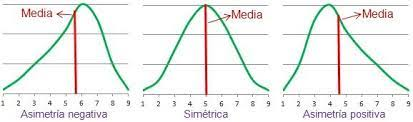
\includegraphics[width=0.5\textwidth]{imagen1.jpeg}
    \caption{negativa = $sk(x) < 0$, Simetrica = $sk(x) = 0$, positiva = $sk(x) > 0$}
    \label{fig:imagen1}
\end{figure}

\textbf{Ejemplo 14}

\noindent Muestra que el coeficiente de asimetria es adimensional e invariante a cambios de escala y origen.

\begin{center}
    $sk(ax+c) = sk(x)$
\end{center}

Demostracion:

\noindent Debido a que $m_3$ y $(m_2)^{\frac{3}{2}}$ tienen la misma unidad de medida, sk(x) es adimensional.

\begin{align*}
    sk(ax+c)    & = \frac{1}{(s(ax+c))^3}[\frac{1}{n} \sum_{i=1}^{n}((ax+c) - (a\bar{x}+c))^3] \\
    Media(ax+c) & = aMedia(x) + c                                                              \\
    s(ax+c)     & = |a|s(x)                                                                    \\
                & = \frac{1}{[|a|s(x)]^3}[\frac{a^3}{n}\sum_{i=1}^{n}(x_i-\bar{x})^3]          \\
                & = \frac{a^3}{|a|^3} \frac{1}{s^3}[\frac{1}{n}\sum_{i=1}^{n}(X_i-\bar{x})^3]  \\
                & = \frac{a^3}{|a|^3} sk(x)
\end{align*}

\subsubsection{Curtosis}

\noindent Sean $x_1, \dots, x_n$ observaciones de la variable x. La curtosis de x se define como.

\begin{align*}
    k(x) & = \frac{1}{s^4}[\frac{1}{n}\sum_{i=1}^{n}(x_i - \bar{x})^4] \\
         & = \frac{m_4}{(m_2)^2}
\end{align*}

\subsubsection{Coeficiente de Fisher}

\[
    k_3(x)=k(x)-3
\]

\begin{figure}[htbp]
    \centering
    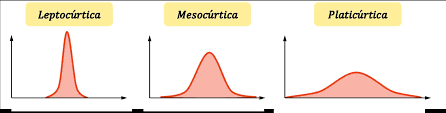
\includegraphics[width=0.7\textwidth]{imagen2.png}
    \caption{}
    \label{fig:imagen2}
\end{figure}

\newpage

\subsection{Medidas de asociacion (1.6.6)}

\begin{figure}[htbp]
    \centering
    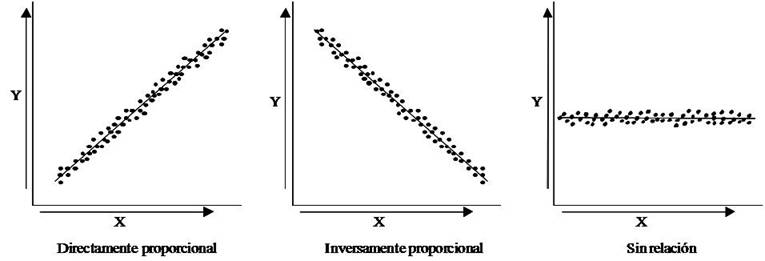
\includegraphics[width=0.7\textwidth]{imagen3.jpg}
    \label{fig:imagen3}
\end{figure}

\subsubsection{Covarianza}

\noindent Sean $(x_1, y_1) \dots, (x_n, y_n)$ observaciones de las variables (x,y). La covarianza entre las variables (x,y) se define como

\[
    s_{xy} = \frac{1}{n}\sum_{i=1}^{n}(x_i-\bar{x})(y_i - \bar{y})
\]

\textbf{Ejemplo 15}

Muestra que

\[
    s_{xy} = \frac{1}{n}[\sum_{i=1}^{n}x_iy_i-n\bar{x}\bar{y}]
\]

\begin{align*}
    s_{xy} & = \frac{1}{n}\sum_{i=1}^{n}(x_i-\bar{x})(y_i - \bar{y})                                                                   \\
           & = \frac{1}{n}\sum_{i=1}^{n}(x_iy_i - x_i\bar{y} - y_i\bar{x} + \bar{x}\bar{y})                                            \\
           & = \frac{1}{n} [\sum_{i=1}^{n}x_iy_i - \sum_{i=1}^{n}x_i\bar{y} - \sum_{i=1}^{n}y_i\bar{x} + \sum_{i=1}^{n}\bar{x}\bar{y}] \\
           & = \frac{1}{n} [\sum_{i=1}^{n}x_iy_i - n\bar{x}\bar{y} - n\bar{x}\bar{y} + n\bar{x}\bar{y}]                                \\
           & = \frac{1}{n}[\sum_{i=1}^{n}x_iy_i - n\bar{x}\bar{y}]
\end{align*}

\begin{center}
    Nota:\\
    $n\bar{x}\bar{y} = n \frac{\sum x_i}{n} \bar{y} = \sum x_i \bar{y}$
\end{center}

\newpage

\subsubsection{Coeficiente de correlacion de Pearson}

\noindent Sean $(x_1, y_1) \dots, (x_n, y_n)$ observaciones de las variables (x,y). El coeficiente de correlacion de Pearson entre las variables (x,y) se define como

\[
    r_xy = \frac{s_{xy}}{s_xs_y}
\]
Donde $s_x$ es la desviacion estandar de x y $s_y$ es la desviacion estandar de y \\

Alguna consideraciones del coeficiente de correlacion son las siguientes:

\begin{center}
    $r_{xy} \in [-1,1]$ \\
    si $x \bot y, r_{xy} = 0$ \\
    si $r_{xy} < 0$, relacion inversa entre las variables
\end{center}

\subsection{Presentacion grafica y tabular de los datos (1.6.7)}

\textbf{Ejemplo 16}

Supongamos que se tiene una variable cualitativa ordinal con valores ordenados de menor a mayor, A,B,C,D,E,F con las siguientes frecuencias,

\begin{table}[h]
    \centering
    \begin{tabular}{|c c c c c|}
        \hline
        Valor & F absoluta & F absoluta acumulada & F relativa & F relativa acumulada \\
        \hline
        A     & 2          & 2                    & 2/28       & 2/28                 \\
        B     & 8          & 10                   & 8/28       & 10/28                \\
        C     & 6          & 16                   & 6/28       & 16/28                \\
        D     & 4          & 20                   & 4/28       & 20/28                \\
        E     & 3          & 23                   & 3/28       & 23/28                \\
        F     & 5          & 28                   & 5/28       & 28/28                \\
        \hline
    \end{tabular}
\end{table}

\newpage

\section{25 agosto 2023}

\subsection{Graficas de barras}

\noindent A cada clase de una variable se le asocia una barra de la altura la frecuencia de las observaciones. Se utiliza para cualquier tipo de variables.

\begin{figure}[htbp]
    \centering
    
\includegraphics[width=0.5\textwidth]{imagen4.png}
    \label{fig:imagen4}
\end{figure}

\subsection{Histograma}

Es una grafica donde los valores de la variable tiene un orden

\begin{figure}[htbp]
    \centering
    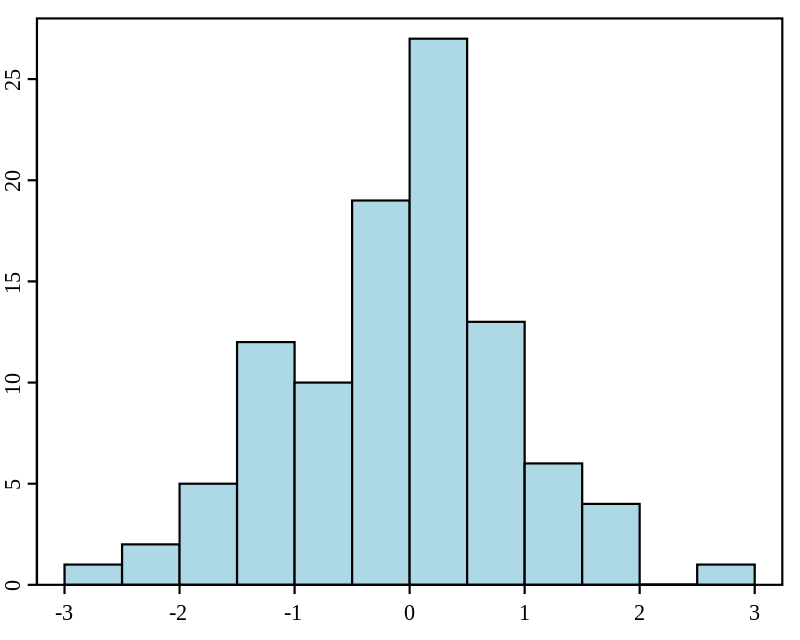
\includegraphics[width=0.5\textwidth]{imagen5.png}
    \label{fig:imagen5}
\end{figure}

\newpage

\subsection{Gráficos de dispersión}

Muestra la relacion entre dos variables

\begin{figure}[htbp]
    \centering
    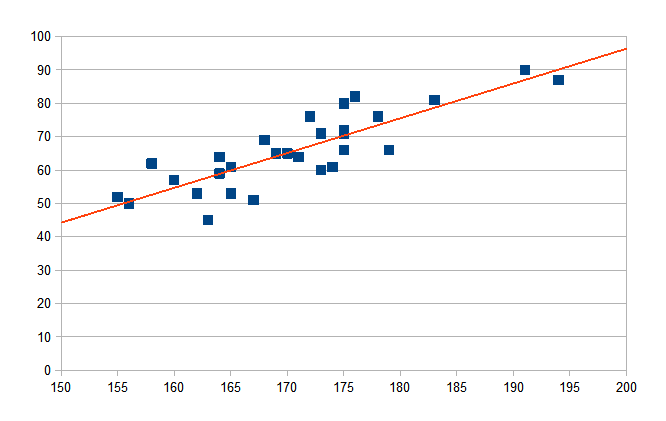
\includegraphics[width=0.5\textwidth]{imagen6.png}
    \label{fig:imagen6}
\end{figure}

\subsection{Gráfica de burbujas}

Muestra la relación para tres variables

\begin{figure}[htbp]
    \centering
    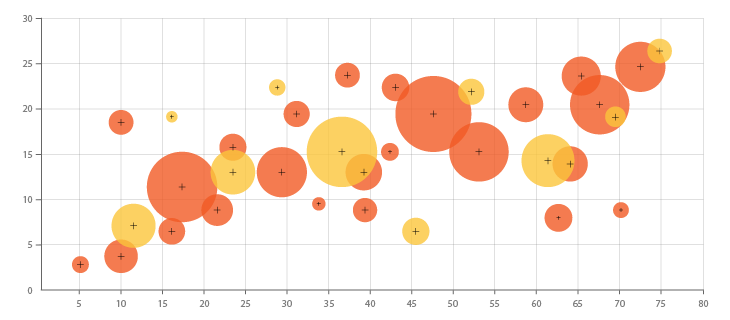
\includegraphics[width=0.6\textwidth]{imagen7.png}
    \label{fig:imagen7}
\end{figure}

\subsection{Serie temporal}

Por medio de una linea se recorren diferentes valores o frecuencias a lo largo del tiempo.

\begin{figure}[htbp]
    \centering
    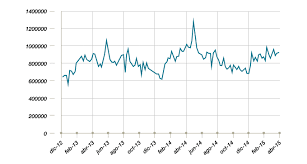
\includegraphics[width=0.6\textwidth]{imagen8.png}
    \label{fig:imagen8}
\end{figure}

\subsection{Introducción a R}

\noindent R es un programa útil para el análisis y visualización de datos. Es abierto y gratuito.

\noindent Es un lenguaje interpretado y tipado.

\noindent Fue creado por Ross lhaka y Robert Gentle-man.

Instalación.

\noindent Descargar R: https://cran.r-project.org/ \\
Descargar R studio: https://posit.co/download/rstudio-desktop/

\subsection{Reglas de sintaxis}

\begin{itemize}
    \item R distingue entre mayúsculas y minúsculas
    \item Los nombres de las variables pueden contener letras, números y puntos. Sin embargo, deben comenzar con una letra y no pueden contener espacion.
          Ejemplo: \\
          Uso correcto \\
          $monto\_total <- 1200$ \\
          $monto\_mensual <- 200$ \\
          Uso incorrecto \\
          $montoTotal <- 1200$ \\
          $MontoMensual <- 200$

    \item Usar espacios alrededor de todos los operadores binarios $(=, +, -, <-, etc)$ y un espacio despúes de una coma.

    \item Ayuda, se puede usar el comando help(mean) o ?mean
    \item Tipos de datos, enteros, númericos y complejos. \\
          Ejemplo: \\
          $entero <- 1L$ \\
          $numerico <- 1$ \\
          $complejo <- 3+4i$ \\
          print(entero, str(entero))
    \item Cadena de texto \\
          Ejemplo: \\
          $mensaje <- "Hola mundo"$ \\
          print(mensaje, str(mensaje))
    \item Factores \\
          Ejemplo: \\
          $colores <- factor(levels = c("azul", "verde"))$ \\
          print(colores)
\end{itemize}

\section{28 agosto 2023}

\subsection{Diagrama de caja y brazos}

\begin{figure}[htbp]
    \centering
    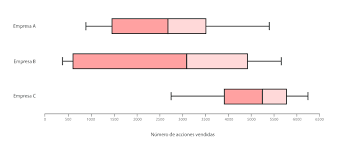
\includegraphics[width=0.6\textwidth]{imagen9.png}
    \label{fig:imagen9}
\end{figure}

\subsection{Continuación de R}

\subsubsection{Operadores aritméticos}

\begin{itemize}
    \item Suma (+)
    \item revista (-)
    \item Multiplicación (*)
    \item División (/)
    \item División entera (\% / \% )
    \item Módulo (\% \%)
\end{itemize}

\subsubsection{Operadores de asignacion}

\begin{itemize}
    \item $valor_1 <- 5$
    \item $valor_2 = 6$
    \item $7 -> valor_3$
\end{itemize}

\subsubsection{Operadores de comparacion e identidad}

\begin{itemize}
    \item Menor
    \item Mayor
    \item Menor o igual
    \item Mayor o igual
    \item Igual
    \item Distinto
\end{itemize}

\subsubsection{Funciones para cadenas de texto}

\begin{itemize}
    \item paste() Concatena varias cadenas en una sola cadena
    \item rep() Repite un objeto n cantidad de veces
    \item grepl() Busca un patron en una cadena de texto y devuelve un vector logico
\end{itemize}

\subsubsection{Listas}

\begin{itemize}
    \item lista <- list(1,"Manzana")
\end{itemize}

\subsubsection{Matrices}

\begin{itemize}
    \item $matriz_1 <- matrix(1:10, nrow=2, ncol=5)$
\end{itemize}

\subsubsection{Convertir tipo de datos}

\begin{itemize}
    \item as.integer
    \item as.numeric
    \item as.complex
    \item as.factor
    \item as.logical
\end{itemize}

\subsection{Funciones con dataFrames}

\begin{itemize}
    \item str()
    \item head()
    \item tail()
    \item summary()
\end{itemize}

\newpage

\section{30 Agosto 2023}

\subsection{Funciones}

\begin{verbatim}
    nombre_funcion <- function(argumentos){
        operaciones
        return(resultado)
    }
\end{verbatim}

\subsection{Unidad 2}

Métodos para la obtención de funciones de variables aleatorias

\vspace{.2cm}

\textbf{Definición}

\vspace{.2cm}

\noindent Consideremos un fenómeno aleatorio junto con un espacio de probabilidad ($\Omega, F, P$). Una variable aleatoria es una transformación $X$ del espacio de resultados $\Omega$ al conjunto de los reales, tal que:

\[
    \{w \in \Omega : X(w) \leq x\} \in F
\]

\vspace{.2cm}

\textbf{Definición}

\vspace{.2cm}

\noindent Una variable aleatoria es discreta cuando el conjunto de valores que toma es un conjunto discreto

\vspace{.2cm}

\textbf{Definición}

\vspace{.2cm}

\noindent Una variable aleatoria en continua cuando el conjunto de valores que toma está en un intervalo $(a,b) \in \mathbb{R}$

\vspace{.2cm}

\textbf{Definición}

\vspace{.2cm}

\noindent Sea $X$ una variable aleatoria discreta con valores $x_0, x_1, \dots$ y probabilidades respectivas $\mathbb{P}(X=x_0), \mathbb{P}(X=x_1), \dots$ la función masa de probabilidad de x denotada por $f(x): \mathbb{R} \rightarrow [0, \infty)$ se define como sigue:

\[
    f(x) = \begin{cases}
        \mathbb{P}(X=x), & \text{si } x = x_1, x_2, \dots, \\
        0,               & \text{c.o.c }.
    \end{cases}
\]

Y cumple con las siguentes Propiedades

\begin{center}
    a) $f(x) \geq 0 \forall x \in \mathbb{R}$ \\
    b) $\sum_{x \in X} f(x) = 1$
\end{center}

\vspace{.2cm}

\textbf{Definición}

\vspace{.2cm}

Sea $X$ una variable aleatoria discreta y $f(x)$ la función masa de probabilidad de $X$, la función de distribución de $X$, denotada por $F(x) \rightarrow [0,1]$ se define como:

\[
    F(x) = \mathbb{P}(X \leq x) = \sum_{x_i\leq x}(f(x_i))
\]

\vspace{.2cm}

\textbf{Definición}

\vspace{.2cm}

Sea $X$ una variable aleatoria continua, decimos que la función integrable $f(x): \mathbb{R} \rightarrow [0, \infty)$ es la función de densidad de $X$ si para cualquier intervalo $(a,b) \in \mathbb{R}$ se cumple que:

\[
    \mathbb{P}(X \in (a,b)) = \int_{a}^{b} f(x) \,dx
\]

y cumple:

\begin{center}
    a)$f(x) \geq 0$ \\
    b)$\int_{-\infty}^{\infty}f(x) = 1$
\end{center}

\vspace{.2cm}

\textbf{Definición}

\vspace{.2cm}

Sea $X$ una variable aleatoria continua y $f(t)$ la función de densidad de $x$, la función de distribución de $X$, denotada por $F(x) = \mathbb{R} \rightarrow [0,1]$, se define como

\[
    F(x) = \mathbb{P}(X \leq x) = \int_{-\infty}^{x}f(t) dt
\]

\vspace{.2cm}

\textbf{Definición}

\vspace{.2cm}

La variable aleatoria $X$ se llama continua si su correspondiente función de distribución es continua y creciente

\vspace{.2cm}

\textbf{Definición}

\vspace{.2cm}

La variable aleatoria $X$ se llama discrtea si su correspondiente función de distribución es constante por pedazos

\vspace{.2cm}

\textbf{Ejemplo}

\vspace{.2cm}

Para cada uno de los siguientes incisos, identifica si la gráfica de la función de distribución corresponde a una variable aleatoria discreta o continua.

\begin{figure}[htbp]
    \centering
    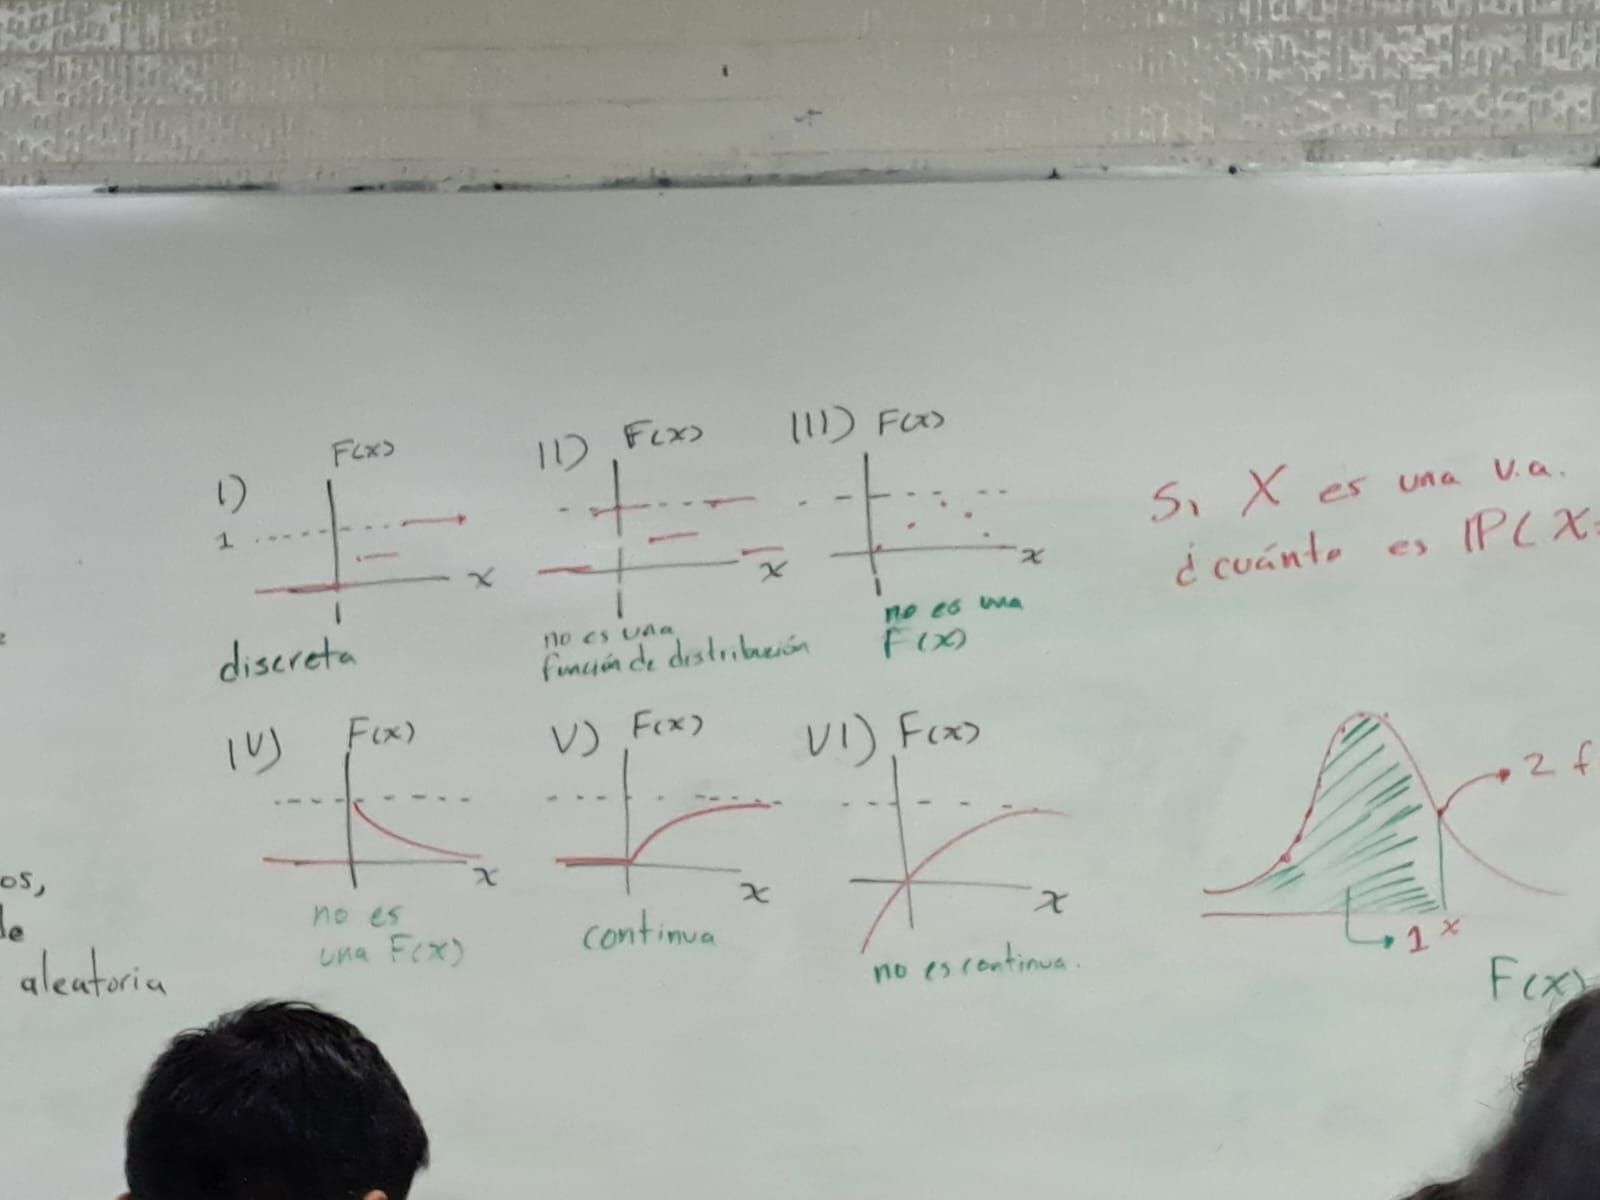
\includegraphics[width=1\textwidth]{Imagen10.jpeg}
    \label{fig:imagen10}
\end{figure}

\newpage

\section{1 Septiembre 2023}

\subsection{Métodos de las funciones de distribución}

\noindent Sea $X$ una variable aleatoria con función de densidad $f(x)$ y $\varphi$ una función de $X$, entonces la variable aleatoria $Y = \varphi(x)$ con funciónde distribución $F_y(y)=\mathbb{P}(Y \leq y)$, $f(y)$ se puede calcular al integrar la región para la cual $Y \leq y$. Ademas, la función de densidad de la variable y se puede calcular al derivar $F_y(y)$\\

\textbf{Ejemplo 2}

Encuentra la función de densidad de la variable $Y$, si $Y=3X-1$ donde.

\[
    f(x) = \begin{cases}
        2x & \text{si } 0 \leq x \leq 1 \\
        0, & \text{c.o.c }.
    \end{cases}
\]

\begin{align*}
    F_y(y) & = \mathbb{P}(Y \leq y)                        \\
           & = \mathbb{P}(3x-1 \leq y)                     \\
           & = \mathbb{P}(3x \leq y + 1)                   \\
           & = \mathbb{P}\left(x \leq \frac{y+1}{3}\right) \\
           & = \int_{0}^{\frac{y+1}{3}} f(x) \, dx
\end{align*}

\begin{itemize}
    \item Si $y=-1$, $\frac{y+1}{3} = 0$
    \item Si $y < -1$ entonces $F_y(y)=0$
    \item Si $y=2$ entonces $F_y(y)=1$
\end{itemize}

\begin{align*}
    F_y(y) & = \int_{0}^{\frac{y+1}{3}} 2x \, dx \\
           & = \frac{(y+1)^2}{9}                 \\
\end{align*}

\[
    F_y(y) = \begin{cases}
        0                  & \text{si } y < -1 \\
        \frac{(y+1)^2}{9}, & -1 \leq y \leq 2  \\
        1                  & \text{si }  y > 2
    \end{cases}
\]

Si derivamos $\frac{d(F_y(y))}{dy}$

\[
    f_y(y) = \begin{cases}
        \frac{2}{9} (y+1)^2 & \text{si } -1 \leq y \leq 2 \\
        0                   & \text{c.o.c}
    \end{cases}
\]

\textbf{Ejemplo 3}

La función de densidad conjunta de $X_1$ y $X_2$ está dada por

\[
    f(x_1, x_2) = \begin{cases}
        3x_1 & \text{si } -0 \leq x_2 \leq x_1 \leq 1 \\
        0    & \text{c.o.c}
    \end{cases}
\]

Encuentra la función de densidad $Y=x_1 - X_2$

\begin{align*}
    F_y(y) & = \mathbb{P}(Y \leq y)                                       \\
           & = \mathbb{P}(X_1 - X_2 \leq y)                               \\
           & = 1 - \mathbb{P}(X_1 - X_2 \leq y)                           \\
           & = 1 - \int_{y}^{1} \int_{0}^{X_1-y} f(x_1, x_2) \, dx_2 dx_1 \\
           & = 1 - \int_{y}^{1} \int_{0}^{X_1-y} 3x_1 \, dx_2 dx_1        \\
           & = 1 - \int_{y}^{1} [3x_1x_2 |_{0}^{x_1-y}] dx_1              \\
           & = 1 - \int_{y}^{1} [3x_1(x_1-y)] dx_1                        \\
           & = 1 - \int_{y}^{1} [3x_1^2 - 3x_1y] dx_1                     \\
           & = 1 - [x_1^3 - \frac{3}{2} x_1^2y |_{y}^{1}]                 \\
           & = 1 - [ 1 - \frac{3}{2}y - (y^3 - \frac{3}{2}y^3)]           \\
           & = [1 - \frac{3}{2}y + \frac{1}{2}y^3]                        \\
           & = \frac{3}{2}y - \frac{1}{2}y^3                              \\
           & = \frac{1}{2}(3y - y^3)
\end{align*}

\subsection{Teorema de cambio de variable}

Sea X una variable aleatoria continua con valores en el intervalo $(a,b) \in \mathbb{R}$ y con función de densidad $f_x(x)$. Sea $\varphi(a,b) \rightarrow \mathbb{R}$ una función continua, estrictamente creciente o decreciente y con inversa. Entonces la variable aleatoria $Y = \varphi$ toma valores en el intervalo $\varphi(a,b)$ y tiene función de densidad

\[
    f(x_1, x_2) = \begin{cases}
        f_x(\varphi^{-1}(y))|\frac{d(\varphi^{-1}(y))}{dy}| & \text{si } y \in \varphi(a,b) \\
        0                                                   & \text{c.o.c}
    \end{cases}
\]

\textbf{Ejemplo 4}

Sea $x \backsim Unif(0,1)$ y $\varphi(x) = \frac{1}{\lambda} \ln(x) = y$ obten $f_y(y)$

\[
    f_x(x) = \begin{cases}
        1 & \text{si } 0 \leq x \leq 1 \\
        0 & \text{c.o.c}
    \end{cases}
\]

\begin{itemize}
    \item Si $x = 1$, $\varphi(1) = -\frac{1}{\lambda} \ln(1) = 0$ \\
    \item Si $x = 0$, $\varphi(0) = -\frac{0}{\lambda} \ln(0) = \infty$ \\
\end{itemize}

Para obtener $\varphi^{-1}(y)$, se tiene que:

\begin{align*}
    -\frac{1}{\lambda} \ln(x) & = y                                           \\
    \ln(x)                    & = - \lambda y                                 \\
    x                         & = e^{-\lambda y}                              \\
                              & = \mathbb{P}\left(x \leq \frac{y+1}{3}\right) \\
                              & = \int_{0}^{\frac{y+1}{3}} f(x) \, dx
\end{align*}

\newpage
\section{08 de Septiembre del 2023}

\subsection{Método de la función generadora de momentos}

\textbf{Definición}

El valor esperado o esperanza de la variable aleatoria de $X$, denotada por $E(x)$ es.

\[
    E(x) = \begin{cases}
        f\int_{-\infty}^{\infty}xf(x)dx & \text{si } X es una v.a.c \\
        \sum_{x}xf(x)                   & \text{si } X en us v.a.d
    \end{cases}
\]

\textbf{Definición}

La varianza de la variable aleatoria $X$ se define como:

\begin{align*}
    var(x) & = E[x-E(x)]^2               \\
           & = E[x^2-2xE(x)+E^2(x)]      \\
           & = E(x^2) - 2E(x)E(x)+E^2(x) \\
           & = E(x^2)-2E^2(x)+E^2(x)     \\
           & = E(x^2) - E^2(x)
\end{align*}

\textbf{Definición}

Sea $X$ una variable aleatoria continua con media $\mu$, el k-ésimo momento central de $X$ es

\[
    m_k = \int_{-\infty}^{\infty}(x-\mu)^kf(x)dx
\]

\textbf{Definición}

Sea $X$ una variable aleatoria, la función generadora de momentos es:

\[
    M_x(t) = E(e^tx)
\]

\textbf{Ejemplo 6}

*Insertar las fotos del ejercicio 6 y 7*

\textbf{Ejemplo 8}

\begin{align*}
    -M_x(t)                           & = \sum_{n=0}^{\infty}\frac{t^n}{n!} E(X^n) \\
    -\frac{d^n[M_x(t)]}{dt^n} |_{t=0} & = E(x^n)                                   \\
\end{align*}

Si $X$ y $Y$ son independientes. Entonces $M_{x+y}(t) = M_x(t) \cdot M_y(t)$

Si $M_x(t) = M_y(t)$ para todos los valores de $t$, entonces $X$ y $Y$ tienen la misma función de distribución

pregunta de examen: si ya conoces la función de densidad y como se identificara la moda?

\section{13 de Septiembre del 2023}

\textbf{Ejemplo 8}

Muestra que si $X \backsim N (\mu, G^2)$, entonces $Y=\frac{X-\mu}{G} \backsim N(0,1)$

Si $N \backsim (\mu G^2)$, entonces $M_x(t) = e(\mu t + \frac{G^2 t^2}{2})$

Si $Y \backsim N(0,1)$

$M_y(t) = e^{\frac{t^2}{2}}$

De manera que

\begin{align*}
    M_y(t) & = E(e^{ty})                                                                  \\
           & = E(e^{t \frac{x-\mu}{G}})                                                   \\
           & = E(e^{\frac{tx}{G}}) E(e^{-\frac{t \mu}{G}})                                \\
           & = e^{-\frac{t \mu}{G}} E(e^{\frac{t}{G}x})                                   \\
           & = e^{-\frac{t \mu}{G}} M_x(\frac{t}{G})                                      \\
           & = e^{-\frac{t \mu}{G}} [e^{\mu \frac{t}{G} + \frac{G^2}{2} \frac{t^2}{G^2}}] \\
           & = e^{-\frac{t \mu}{G} + \frac{t \mu}{G} + \frac{t^2}{2}}
           & = e^{\frac{t^2}{2}}
\end{align*}

\section{18 de Septiembre del 2023}

\textbf{Ejemplo 11}

Sea $X \backsim Exp(1/100)$. Encuentra $f_{x(1)}(x)$ para una muestra de tamaño 2.

\begin{align*}
    f_{x(1)}(x) & = nf_{(x)}[1-F_{(x)}]^{n-1}                  \\
    \text{Si $X \backsim Exp(1/100)$}                          \\
    f(x)        & = 100 exp^{-100x}                            \\
    F(x)        & = 1- exp^{-100x}                             \\
    n           & = 2                                          \\
    f_{x(1)}(x) & = 2 (100 exp^{-100x})(1-1+exp^{-100x})^{2-1} \\
                & = 200 exp^{-200x}
\end{align*}

por lo tanto: $f_{x(1)}(x) \backsim Exp(\beta = 1/200)$

\subsection{Distribuciones derivadas de la normal}

\subsubsection{Normal estándar}

Si $X \backsim N(0,1)$ se dice que $x$ que se distribuye como una normal estándar.

\textbf{Propiedades}

\begin{itemize}
    \item La media, la mediana y la moda son iguales a $\mu$
    \item El $68\%$ de las observaciones caen en el intervalo $[\mu - \sigma, \mu + \sigma]$
    \item El $95\%$ de las observaciones caen en el intervalo $[\mu - 2\sigma, \mu + 2\sigma]$
    \item El $99.7\%$ de las observaciones caen en el intervalo $[\mu - 3\sigma, \mu + 3\sigma]$
    \item $\mathbb{P}(-1 \leq x \leq 1) = 68\%$
    \item $\mathbb{P}(x \leq 0) = 50\%$
    \item $\mathbb{P}(x = 0) = 0\%$
    \item $\mathbb{P}(0 \leq x \leq 1) = 34\%$
\end{itemize}

\subsubsection{Ji cuadrada}

Sean $Z_1, \cdots, Z_k$ variables aleatorias con distribución normal estándar

\[
    x = z_1^2 + \cdots + z_k^2
\]

Entonces, $X \backsim X^2_k$ donde

$E(x) = k$ y $Var(x) = 2k$

\section{Unidad 3}

\textbf{Distribuciones muestrales}

\subsection{Introducción}

\textbf{Definición}

Una muestra aleatoria es una colección de variable aleatoria $X_1, \cdots , X_n$ que cumplen con la condición de ser independientes y de tener cada una de ellas la misma distribución.

\textbf{Definición}

Un estadístico es una variable aleatoria de la forma $g(X_1, \cdots, X_n)$ en donde $X_1, \cdots, X_n$ es una muestra aleatoria y $g: \mathbb{R}^n \rightarrow \mathbb{R}$

Por ejemplo, la media muestral es un estadístico al igual que la varianza muestral

\textbf{Definición}

Dado que los estadísticos son funciones de variables aleatorias entonces los estadísticos tienen funciones de probabilidad que se denominan Distribuciones muestrales.

\textbf{Definición}

Un párametro es una caracterización numérica de la población de manera que describe parcialmente la función de la probabilidad.
\begin{center}
    \begin{tabular}{|c|c|}
        \hline
        población  & Muestra   \\
        \hline
        N          & n         \\
        $\mu$      & $\bar{x}$ \\
        $\sigma^2$ & $s^2$     \\
        \hline
    \end{tabular}
\end{center}

\textbf{Proposición}

Sea $X_1, \cdots, X_n$ una muestra aleatoria con función generadora de momentos $M_{x1}(t), \cdots, M_{xn}(t)$ y
\[
    y=a_1X_1 + \cdots + a_nX_n
\]

En donde $a_1, \cdots, a_n$ son constantes, entonces.

\[
    M_y(t) = M_{x1}(a_1t) \cdots M_{xn}(a_nt)
\]

\textbf{Ejemplo 1}

Sea $X_1, \cdots, X_n$ una muestra aleatoria con distribución normal donde $E(x_i) = \mu_i$ y $Var(X_i) = \sigma_i^2$, $i=1, \cdots, n$. Si $Y = a_1X_1 + \cdots + a_nX_n$, muestra que $Y$ se distribuye como una normal.

Si $X_i \sim N(\mu_i, \sigma_i^2)$

entonces

\[
    M_{xi}(t) = e^{\mu_i t + \frac{\sigma^2_i t^2}{2}}
\]

\[
    M_{xi}(t) = e^{\mu_i a_it + \frac{a_i^2 \sigma^2_i t^2}{2}}
\]

\section{22 de Septiembre del 2023}

\subsection{Distribución de muestreo de $\bar{X}$}

Sea $X_1, \cdots, x_n$ una muestra aleatoria tal que $E(x_i) = \mu$ y $Var(x_i) = \sigma^2$ para $i = 1, \cdots, n$. Entonces

\[
    E(\bar{X}) = \mu
\]

\[
    Var(\bar{X}) = \frac{\sigma^2}{n}
\]

\textbf{Demostración}

\begin{align*}
    E(\bar{X}) & = E(\frac{1}{n}\sum_{i=1}^{x_i})        \\
               & = E(\frac{1}{n}[x_1, \cdots, c_n])      \\
               & = \frac{1}{n}(E(x_1) + \cdots + E(x_n)) \\
               & = \frac{1}{n} (\mu + \cdots + \mu)      \\
               & = \frac{n \mu}{n} = \mu                 \\
\end{align*}

\begin{align*}
    Var(\bar{X}) & = Var(\frac{1}{n}\sum_{i=1}^{x_i})             \\
                 & = Var(\frac{1}{n}[x_1, \cdots, c_n])           \\
                 & = \frac{1}{n^2}(Var(x_1) + \cdots + Var(x_n))  \\
                 & = \frac{1}{n^2} (\sigma^2 + \cdots + \sigma^2) \\
                 & = \frac{n \sigma^2}{n^2} = \frac{\sigma^2}{n}  \\
\end{align*}

\textbf{Ejemplo 3}

Sea $X_1, \cdots, x_n$ v.a.i.i.d con distribución normal donde $E(x_1) = 3.25$, $E(x_2) = 3.3$, $\sqrt{Var(x_1)} = 0.005$ y $\sqrt{Var(x_2)} = 0.006$

Sea $y = x_2 - x_1$. Calcula $E(y)$ y $Var(y)$

\[
    E(y) = E(x_2 - x_1) = E(x_2) - E(x_1) = 3.3 - 3.25 = 0.05
\]

\[
    Var(y) = Var(x_2 - x_1) = Var(X_2) + Var(x_1) = (0.000061)^2 + (0.005)^2 = 0.000061
\]

Si $z \sim x_4^2$

$\mathbb{P}(z > 4) = \mathbb{P}(\frac{z-E(z)}{\sqrt{Var(z)}} > \frac{4-E(z)}{\sqrt{Var(z)}}) = \mathbb{P}(\frac{z-4}{\sqrt{8}} > \frac{4-4}{\sqrt{8}}) = \mathbb{P}(x>0)$

\subsection{Teorema central del limite}

Sea $X_1, \cdots, x_n$ una sucesión de v.a.i.i.d. tales que para cada natural n, $E(x_n) = \mu$ y $Var(x_n) = \sigma^2$. Entonces

\[
    \frac{\bar{X} - \mu}{\frac{\sigma}{\sqrt{n}}} \sim N(0,1)
\]

\section{25 de Septiembre del 2023}

\textbf{Ejemplo 4}

Se ha seleccionado una muestra al azar de 50 mujeres de una población de mayores de 18 años. se desconoce la estatura media de la población pero en la muestra observada se obtuvo que $\bar{x} = 1.60$m. Si se sabe por otros estudios que la desviación estandar poblacional es de $0.33$m

Determina la probabilidad de que la media muestral no difiera en más de $0.01$m de la media poblacional.

$\bar{x}$, $E(\bar{x}) = \mu$
\begin{align*}
    (\bar{x}) & = \mu
              & = \bar{x}
              & = 1.60
\end{align*}

\begin{align*}
    \mathbb{P}(|\bar{x} - \mu| < 0.01) & = \mathbb{P}(-0.01 < \bar{x} - \mu < 0.01)                                                                                  \\
                                       & = \mathbb{P}(\frac{-0.01}{\frac{6}{\sqrt{n}}} < \frac{\bar{x} - \mu}{\frac{6}{\sqrt{n}}} < \frac{0.01}{\frac{6}{\sqrt{n}}}) \\
                                       & = \mathbb{P}(\frac{-0.01}{\frac{0.033}{\sqrt{50}}} < z < \frac{0.01}{\frac{0.033}{\sqrt{50}}})                              \\
                                       & = \mathbb{P}(-2.14 < z < 2.14)                                                                                              \\
                                       & = \mathbb{P}(z< 2.14) - \mathbb{P}(z < -2.14)
\end{align*}

\subsection{La distribución de muestreo de $s^2$}

Sean $(x_1, y_1) \dots, (x_n, y_n)$ v.a.i.i con distribución normal con media $\mu$ conocida y varianza $\sigma^2$. Entonces
\[
    \frac{nS^2_n}{\sigma^2} \sim X_n^2
\]

Donde

\[
    S^2_n = \frac{\sum_{i=1}^{n}(x_i-\mu)^2}{n}
\]

\textbf{Ejemplo 5}

Sean $(x_1, y_1) \dots, (x_n, y_n)$ v.a.i.i con distribución $N(\mu = 10, \sigma^2 = 0.01)$. Calcula la probabilidad de que la varianza muestral sea mayor que $0.014$

\begin{align*}
    \mathbb{P}(S^2_n > 0.014)                   & = \mathbb{P}(\frac{nS^2_n}{\sigma^2} > \frac{0.014n}{\sigma^2}) \\
                                                & = \mathbb{P}(X^2_n > \frac{0.014}{0.01}n)                       \\
    \text{Si} n=25                                                                                                \\
    \mathbb{P}(X^2_25 > \frac{0.014(25)}{0.01}) & = \mathbb{P}(X^2_{25} > 35)                                     \\
                                                & = 1 - \mathbb{P}(X^2_n < 35)                                    \\
\end{align*}

En r 1 - pchisq(35,25) = 0.088203

\subsection{Aproximación normal}
\[
    \mathbb{P}(X^2_n > 35)
\]

\section{27 de Septiembre del 2023}

\subsection{Estimacion puntual y por intervalos}

estimador $neq$ Estimacion

\subsection{Propiedades de los estimadores}

\textbf{Definición} Un estimador $\theta$ del parametro $\theta$ se dice que es insesgado si $E(\hat{\theta}) = \theta$

\textbf{Ejemplo 2}

Define el espacio parametral de las siguientes Distribuciones
\[
    Exp(\lambda), H = (0, \infty)
\]
\[
    N(\mu, \sigma^2), H = (-\infty, \infty) x (0, \infty)
\]

\textbf{Definición}
Un estadístico $\theta_n $ basado en una muestra de tamano n es un estimador asintotico insesgado para el parametro $\theta$ si
\[
    lim_{n \rightarrow \infty} E(\theta_n) = \theta
\]

\[
    \mathbb{P}(z \leq 0.41) = 0.6591
\]

\textbf{Definición}. Sea $\hat{\theta_n}$ un estimador para el parametro $\theta$, basado en una muestra de tamaño n, $\hat{theta_n}$ es consistente si para cualquier $\epsilon > 0$

\section{2 de Octubre del 2023}

\subsection{Métodos para obtener estimadores puntuales}

\subsubsection{Método de momentos}

Consiste en igualar los momentos poblacionales con los correspondientes momentos muestrales y resolver esta ecuación o sistema de ecuaciones para el parámetro o vector de párametros desconocidos.

\[
    E(x) \backsimeq \frac{1}{n} \sum_{i=1}^{n} x_i = \bar{x}
\]
\[
    E(x^2) = \frac{1}{n} \sum_{i=1}^{n}x_i^2
\]

Si $X$ es una v.a continua
\[
    E(x^j) = \int_{-\infty}^{\infty} x^j f(x)dx
\]

Por ejemplo, si $X \backsim N(\mu, \sigma^2)$

\[
    E(x) = \mu
\]

\textbf{Ejemplo 4}

Sea $X$ una variable aleatoria con funcion de densidad

\[
    f(x) = \begin{cases}
        \theta x^{\theta - 1} & \text{si } 0 \leq x \leq 1 \\
        0                     & \text{eoc }
    \end{cases}
\]

Utiliza el metodo de momentos para estimar $\theta$

\begin{align*}
    E(x) & = \int_{-\infty}^{\infty} xf(x) dx                        \\
         & = \int_{-1}^{1}x \theta x^{\theta - 1}                    \\
         & = \int_{-1}^{1}\theta x^\theta dx                         \\
         & = \frac{\theta}{\theta + 1}x^{\theta + 1} \bigg|_{-1}^{1} \\
         & = \frac{\theta}{\theta + 1}
\end{align*}

Por lo tanto

\[
    \frac{\hat{\theta}}{\hat{\theta} + 1} = \bar{x}
\]

\[
    \hat{\theta} = \frac{\bar{x}}{1 - \bar{x}}
\]

\textbf{Ejemplo 5}

Sea $X_1, \cdots X_n$ una muestra aleatoria con distribución $N(\mu, \sigma^2)$ usa el metodo de momentos para estimar $\mu$ y $\sigma^2$

\[
    E(x) = \frac{1}{n} \sum x_i
\]

\[
    E(x^2) = \frac{1}{n} \sum x_i^2
\]

\[
    \mu = \bar{x}
\]

Por otro lado

\begin{align*}
    E(x^2) & = var(x) + E(x^2)                     \\
           & = \sigma^2 + \mu^2                    \\
           & = \int_{-\infty}^{\infty} x^2 f(x) dx \\
\end{align*}

\begin{align*}
    \hat{\sigma^2} + \hat{\mu^2} & = \frac{1}{n} \sum x_i                        \\
    \hat{\sigma^2} + \bar{x}^2   & = \frac{1}{n} \sum x_i                        \\
    \sigma^2                     & = \frac{1}{n}\sum x_i - \bar{x}^2             \\
    \sigma^2                     & = \frac{1}{n} \sum_{i=1}^{n}(x_i - \bar{x})^2
\end{align*}

Insertar imagen del 2 de Octubre

Insertar ejemplo 6

\section{4 de Octubre del 2023}

\textbf{Ejemplo 7}

\[
    L(\beta | x) = \prod_{i=1}^{n} f(x_i | \beta)
\]

\[
    = \frac{1}{\beta^n} e^{-\sum x_i / \beta}
\]

\begin{align*}
    \log[L(\beta | x)] & = \log[\frac{1}{\beta^n} e^{-\sum x_i / \beta}]         \\
                       & = \log[\frac{1}{\beta^n}] + \log[e^{-\sum x_i / \beta}] \\
                       & = \log[\beta^{-n}] - \frac{\sum x_i}{\beta}             \\
                       & = -n\log(\beta) - \sum x_i \beta^{-1}                   \\
\end{align*}

\textbf{Ejemplo 8}

Sea $X_1, \cdots X_2$ una m.a que se distribuye como una $N(\mu, \sigma^2)$. Utiliza ek método de máxima verisimilitud para encontrar $\hat{\mu}$, $\hat{\sigma^2}$

\begin{align*}
    L(\mu,\sigma^2 |x) & = \prod_{i=1}^{n}f(\mu, \sigma^2 | x_i)                                                \\
                       & = \prod_{i=1}^{n}\frac{1}{\sqrt{2\pi \sigma^2}} e^{\frac{-(x_i - \mu)^2}{2\sigma^2}}   \\
                       & = \prod_{i=1}^{n} (2 \pi \sigma^2)^{-\frac{1}{2}} e^{\frac{-(x_i - \mu)^2}{2\sigma^2}} \\
                       & = (2\pi \sigma)^{-\frac{n}{2}} e^{-\frac{\sum(x_i - \mu)^2}{2\sigma^2}}
\end{align*}

\begin{align*}
    \log[L(\mu,\sigma^2 |x)] & = \log\left[(2\pi \sigma)^{-\frac{n}{2}} e^{-\frac{\sum(x_i - \mu)^2}{2\sigma^2}}\right]                      \\
                             & = \log\left[(2\pi \sigma^2)^{-\frac{n}{2}}\right] + \log\left[e^{-\frac{\sum(x_i - \mu)^2}{2\sigma^2}}\right] \\
                             & = -\frac{n}{2} \log(2\pi \sigma^2) - \frac{\sum(x_i - \mu)^2}{2\sigma^2}.
\end{align*}

\[
    \frac{d \log[L(\mu,\sigma^2 |x)]}{d\mu}
\]
Para resolver la derivada con respecto a \( \mu \) de la log-verosimilitud de una distribución normal, primero recordemos la expresión para \( \log[L(\mu,\sigma^2 |x)] \):

\[
    \log[L(\mu,\sigma^2 |x)] = -\frac{n}{2} \log(2\pi \sigma^2) - \frac{\sum(x_i - \mu)^2}{2\sigma^2}
\]

Ahora, vamos a derivar con respecto a \( \mu \):

\[
    \frac{d \log[L(\mu,\sigma^2 |x)]}{d\mu} = \frac{d}{d\mu} \left(-\frac{n}{2} \log(2\pi \sigma^2) - \frac{\sum(x_i - \mu)^2}{2\sigma^2}\right)
\]

El primer término, \( -\frac{n}{2} \log(2\pi \sigma^2) \), no depende de \( \mu \), por lo que su derivada es 0.

El segundo término, centrémonos en derivar \( -\frac{\sum(x_i - \mu)^2}{2\sigma^2} \) con respecto a \( \mu \):

\[
    \frac{d}{d\mu} \left(-\frac{\sum(x_i - \mu)^2}{2\sigma^2}\right) = -\frac{1}{2\sigma^2} \sum 2(x_i - \mu)(-1) = \frac{\sum(x_i - \mu)}{\sigma^2}
\]

Por lo tanto, la derivada de la log-verosimilitud con respecto a \( \mu \) es:

\[
    \frac{d \log[L(\mu,\sigma^2 |x)]}{d\mu} = \frac{\sum(x_i - \mu)}{\sigma^2}
\]

Esta derivada nos da la tasa de cambio de la log-verosimilitud con respecto a \( \mu \). Para encontrar el valor de \( \mu \) que maximiza la log-verosimilitud (y, por lo tanto, la verosimilitud), podemos resolver para \( \mu \) cuando esta derivada es igual a cero. Este proceso nos dará el estimador de máxima verosimilitud (MLE) para \( \mu \) en una distribución normal.

\[
    \begin{cases}
        \frac{\sum(x_i - \hat{\mu})}{\sigma^2} = 0 \\
        -\frac{n}{2\sigma^2} + \frac{\sum (x_i - \mu)^2}{2(\sigma^2)^2} = 0
    \end{cases}
\]

Vamos a resolver el sistema de ecuaciones que nos has dado paso a paso.

Dadas las ecuaciones: \\
1) \[\frac{\sum(x_i - \hat{\mu})}{\sigma^2} = 0\]
2) \[-\frac{n}{2\sigma^2} + \frac{\sum (x_i - \mu)^2}{2(\sigma^2)^2} = 0\]

**Resolviendo la primera ecuación:**
De la ecuación (1), tenemos:
\[ \sum(x_i - \hat{\mu}) = 0 \]
Sumando todos los \( x_i \) y reorganizando los términos, tenemos:
\[ \sum x_i = n\hat{\mu} \]
De aquí, podemos deducir que:
\[ \hat{\mu} = \frac{\sum x_i}{n} \]
Esto es simplemente el promedio de los valores de \( x_i \).

**Resolviendo la segunda ecuación:**
La ecuación (2) es:
\[ -\frac{n}{2\sigma^2} + \frac{\sum (x_i - \mu)^2}{2(\sigma^2)^2} = 0 \]
Multiplicando todo por \(2(\sigma^2)^2\):
\[ -n\sigma^2 + \sum (x_i - \mu)^2 = 0 \]
Reorganizando, obtenemos:
\[ \sum (x_i - \mu)^2 = n\sigma^2 \]
Dividimos ambos lados por \( n \):
\[ \frac{\sum (x_i - \mu)^2}{n} = \sigma^2 \]

Aquí, \(\sigma^2\) es simplemente la varianza de los valores de \( x_i \).

Por lo tanto, las soluciones para el sistema de ecuaciones son:
\[ \hat{\mu} = \frac{\sum x_i}{n} \]
\[ \sigma^2 = \frac{\sum (x_i - \mu)^2}{n} \]

\textbf{Teorema Cota inferior de Cramér-Rao}

Sea $X_1, \cdots X_n \backsim f(x | \theta)$, $\theta \in $
Sea $T$ un estimador de $\theta$ y

\[
    Var(T) \geq \frac{1}{nE[\frac{d \log(f(x|\theta))}{d\theta}]^2}
\]

Si $T$ es insesgado para $\theta$ y $Var(T) = CICR((\theta))$. $T$ es UMVUE (Estimador, insesgado de minima varianza)

\textbf{Ejemplo 9}

Calcula el $CICR(\theta)$ para el modelo Bernoulli\\

Recordemos que una variable aleatoria \( X \) sigue una distribución Bernoulli con parámetro \( \theta \) si su función de masa de probabilidad (fmp) es:

\[ P(X=k|\theta) = \theta^k (1-\theta)^{1-k} \]

para \( k \in \{0,1\} \) y \( 0 < \theta < 1 \).

Para calcular la Cota Inferior de Cramér-Rao, primero necesitamos encontrar la información de Fisher \( I(\theta) \). La información de Fisher para una muestra es:

\[ I(\theta) = E\left[ \left(\frac{\partial \ln f(X;\theta)}{\partial \theta}\right)^2 \right] \]

Calculemos primero la derivada del logaritmo de la fmp respecto de \( \theta \).

Dada:
\[ \ln f(X | \theta) = \ln(\theta^x) + \ln((1-\theta)^{1-x}) \]
\[ \ln f(X | \theta) = x \ln(\theta) + (1-x) \ln(1-\theta) \]

Derivando con respecto a \( \theta \) obtenemos:

\[ \frac{\partial \ln f(X|\theta)}{\partial \theta} = \frac{x}{\theta} - \frac{1-x}{1-\theta} \]

Elevando al cuadrado esta derivada:

\[ \left( \frac{\partial \ln f(X|\theta)}{\partial \theta} \right)^2 = \left(\frac{x}{\theta} - \frac{1-x}{1-\theta}\right)^2 \]
Pedirle a chatgpt concluir
El profe conluyo $CICR(\theta) = \frac{\theta(1-\theta)}{n}$

\textbf{Ejemplo 10}

Muestar que $\hat{\theta} = \bar{x}$ es UMVUE para una m.a con distribucion $Bern(\theta)$

\section{11 de Octubre del 2023}

\textbf{Ejemplo}

Muestra que la media muestral es UMVUE para el parametro $\beta$ de una exponencial

Cuota inferior de Cramér-Rao

\[CICR(\theta) = \frac{1}{nE\left[\frac{d[Ln(f(X|\theta))]}{d\theta}\right]^2}\]

Funcion de dednsidad exponencial

\[f(x|\beta) = \frac{1}{\beta}e^{-x/\beta}\]

Primero, calculemos el logaritmo de esta función:

\[\ln\left(\frac{1}{\beta}e^{-\frac{x}{\beta}}\right) = -\ln(\beta) - \frac{x}{\beta}\]

Ahora, calculamos su derivada con respecto de $\beta$

\begin{align*}
    E\left[\frac{d Log(f(x|\beta))}{d\beta}\right]^2 & = E\left[-\frac{1}{\beta} + \frac{x}{\beta^2}\right]^2                       \\
                                                     & = E\left[\frac{x}{\beta^2} - \frac{1}{\beta}\right]^2                        \\
                                                     & = E\left[\frac{x^2}{\beta^4} - \frac{2x}{\beta^3} + \frac{1}{\beta^2}\right]
\end{align*}

Sabemos que

\[Var(x) = \beta^2 \hspace*{1cm} E(x) = \beta\]

Entonces al distribuir la esperanza tenemos:

Nota: $\beta$ es una constante por lo tanto solo no fijamos en $x$

\[\frac{E[x^2]}{\beta^4} - \frac{E[2x]}{\beta^3} + \frac{1}{\beta^2}\]

para calcular $E[x^2]$ podemos observar la varianza y despejar el valor de $E[x^2]$

\begin{align*}
    Var(x) & = E[x^2] - E^2[x] = \beta^2  \\
           & = E[x^2] - \beta^2 = \beta^2 \\
           & = E[x^2] = 2\beta^2
\end{align*}

por lo tanto

\[\frac{2\beta^2}{\beta^4} - \frac{2\beta}{\beta^3} + \frac{1}{\beta^2} = \frac{1}{\beta^2}\]

\[CIRC(\beta) = \frac{1}{n\frac{1}{\beta^2}} = \frac{\beta^2}{n}\]

\begin{align*}
    E(\bar{x}) & = E(\frac{1}{n} \sum_{i=1}^{n} x_i)                 \\
               & = \frac{1}{n} E(x_1 + \cdots + x_n)                 \\
               & = \frac{1}{n} \left[E(x_1) + \cdots + E(x_n)\right] \\
               & = \frac{1}{n} [n\beta]                              \\
               & = \beta
\end{align*}

\begin{align*}
    Var(\bar{x}) & = Var(\frac{1}{n} \sum_{i=1}^{n} x_i)                 \\
                 & = \frac{1}{n^2} Var(x_1 + \cdots +  x_n)              \\
                 & = \frac{1}{n^2} \left[Var(x_1) \cdots Var(x_n)\right] \\
                 & = \frac{1}{n^2} [n\beta^2]                            \\
                 & = \frac{\beta^2}{n}
\end{align*}

Como $\bar{x}$ es insesgada y $Var(\bar{x}) = \frac{\beta^2}{n} = CIRC(\beta)$, entonces $\bar{X}$ es UMVUE

\section{13 de Octubre del 2023}

\textbf{Teorema de factorizacion}
Un estadistico $T = \tau(X_1, \cdots, X_n)$es suficiente para $\theta$ si y solo si, $L(\theta|X)$ se puede escribir como

\[g(T(X|\theta))h(X)\]

\textbf{Ejemplo 12}

Muestra que $T = \sum_{i=1}^{n}x_i$ es suficiente para $f(X|\theta) = \theta^x(1-\theta)^{1-x}$

\begin{align*}
    L(\theta | x) & = \prod_{i=1}^{n}f(x_i|\theta)
\end{align*}

\newpage

\section{16 de octubre del 2023}

\begin{figure}[htbp]
    \centering
    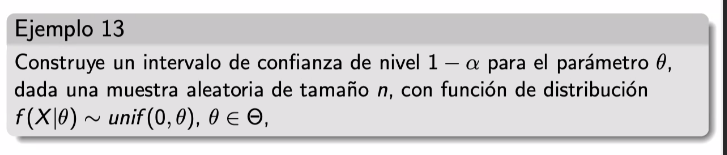
\includegraphics[width=1\textwidth]{Imagen16.png}
    \label{fig:imagen16}
\end{figure}

\begin{figure}[htbp]
    \centering
    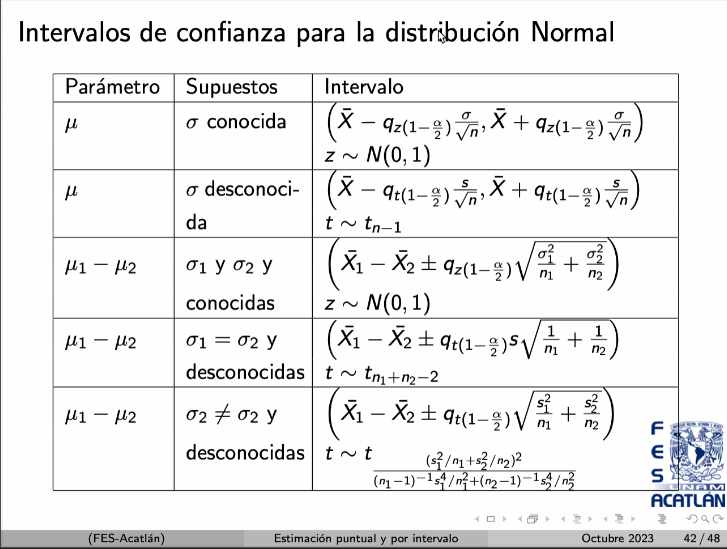
\includegraphics[width=1\textwidth]{Imagen17.png}
    \label{fig:imagen17}
\end{figure}

\begin{figure}[htbp]
    \centering
    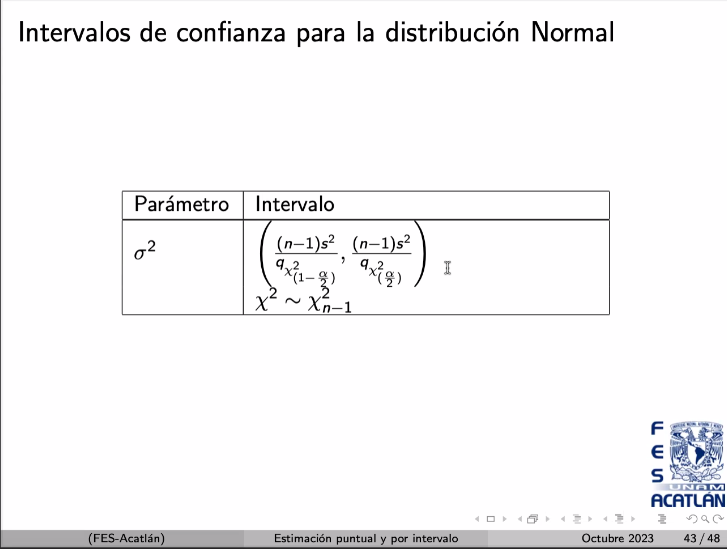
\includegraphics[width=1\textwidth]{Imagen18.png}
    \label{fig:imagen18}
\end{figure}

\begin{figure}[htbp]
    \centering
    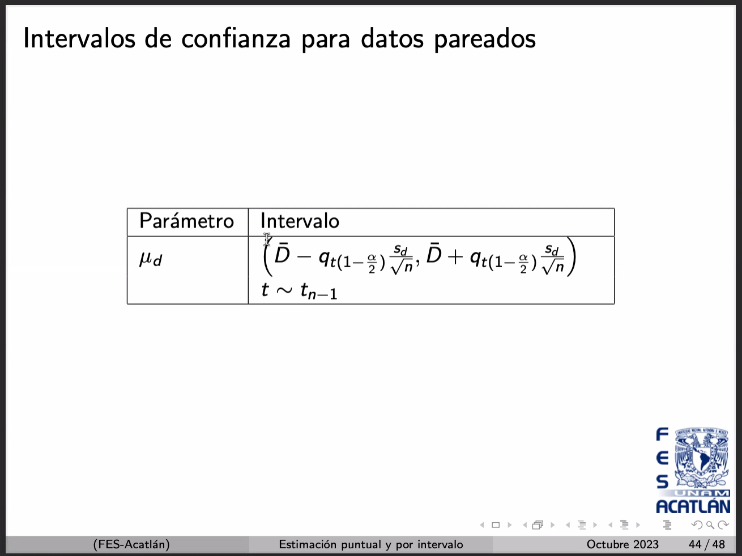
\includegraphics[width=1\textwidth]{Imagen19.png}
    \label{fig:imagen19}
\end{figure}

\begin{figure}[htbp]
    \centering
    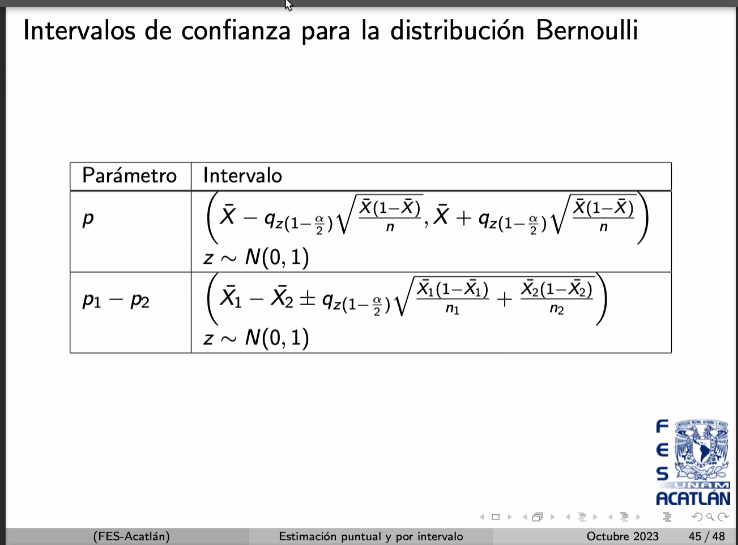
\includegraphics[width=1\textwidth]{Imagen20.png}
    \label{fig:imagen20}
\end{figure}

\begin{figure}[htbp]
    \centering
    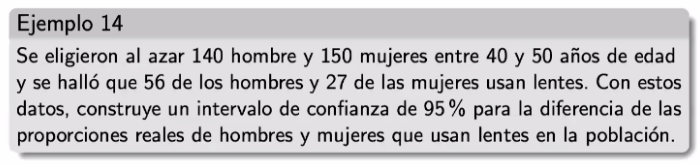
\includegraphics[width=1\textwidth]{Imagen21.png}
    \label{fig:imagen21}
\end{figure}

\clearpage

Primero, identificamos los datos: \\

\noindent \( n_1 \) = número de hombres = 140 \\
\( n_2 \) = número de mujeres = 150 \\
\( x_1 \) = número de hombres que usan lentes = 56 \\
\( x_2 \) = número de mujeres que usan lentes = 27 \\

De aquí, podemos encontrar las proporciones muestrales:

\[ x_1 = \frac{x_1}{n_1} = \frac{56}{140} = 0.4 \]
\[ x_2 = \frac{x_2}{n_2} = \frac{27}{150} = 0.18 \]

La diferencia de proporciones muestrales es:
\[ x_1 - x_2 = 0.4 - 0.18 = 0.22 \]

Para un intervalo de confianza del 95\%, \( z \) es aproximadamente 1.96 (dado que \( z \) sigue una distribución normal estándar).

\[
    q_z(1 - \frac{\alpha}{2}) = q_z(1 - \frac{1 - 0.95}{2})
\]

\[
    q_z(1 - \frac{0.05}{2}) = q_z(1 - 0.025)
\]

\[
    q_z(0.975) = 1.96
\]

Esto se sabe por la tabla z

\begin{figure}[htbp]
    \centering
    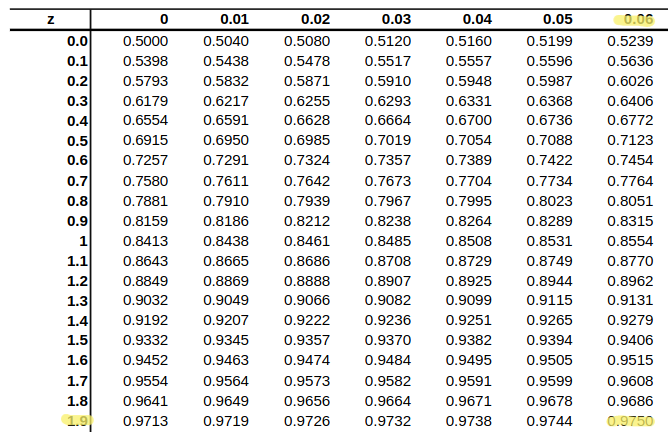
\includegraphics[width=0.6\textwidth]{Imagen22.png}
    \label{fig:imagen22}
\end{figure}

\clearpage

Usando la fórmula dada:
\[ \bar{X}_1 - \bar{X}_2 \pm q_z(1 - \frac{\alpha}{2}) \sqrt{\frac{\bar{X}_1(1-\bar{X}_1)}{n_1} + \frac{\bar{X}_2(1-\bar{X}_2)}{n_2}} \]

Calculamos el margen de error:
\[ ME = 1.96 \sqrt{\frac{0.4(1-0.4)}{140} + \frac{0.18(1-0.18)}{150}} \]
\[ ME = 1.96 \sqrt{\frac{0.24}{140} + \frac{0.1476}{150}} \]
\[ ME \approx 1.96(0.0415) \]
\[ ME \approx 1.96(0.0415) \]
\[ ME \approx 0.08134 \]

Ahora que tenemos el margen de error (ME), podemos calcular el intervalo de confianza para la diferencia de proporciones:

Límite inferior (LI):
\[ LI = x_1 - x_2 - ME \]
\[ LI = 0.22 - 0.08134 \]
\[ LI \approx 0.13866 \]

Límite superior (LS):
\[ LS = x_1 - x_2 + ME \]
\[ LS = 0.22 + 0.08134 \]
\[ LS \approx 0.30134 \]

Por lo tanto, el intervalo de confianza del 95\% para la diferencia de las proporciones reales de hombres y mujeres que usan lentes en la población es:

\[ (0.13866, 0.30134) \]

Esto significa que, con un 95\% de confianza, la diferencia real entre las proporciones de hombres y mujeres que usan lentes se encuentra en el rango de 13.866\% a 30.134\%.

\newpage

\textbf{Ejemplo 1}
Se elabora un examen de 10 preguntas de opcion multiple. Cada pregunta tieme cinco posibles respuestas. Calcula $\alpha$ y $\beta$

\begin{figure}[htbp]
    \centering
    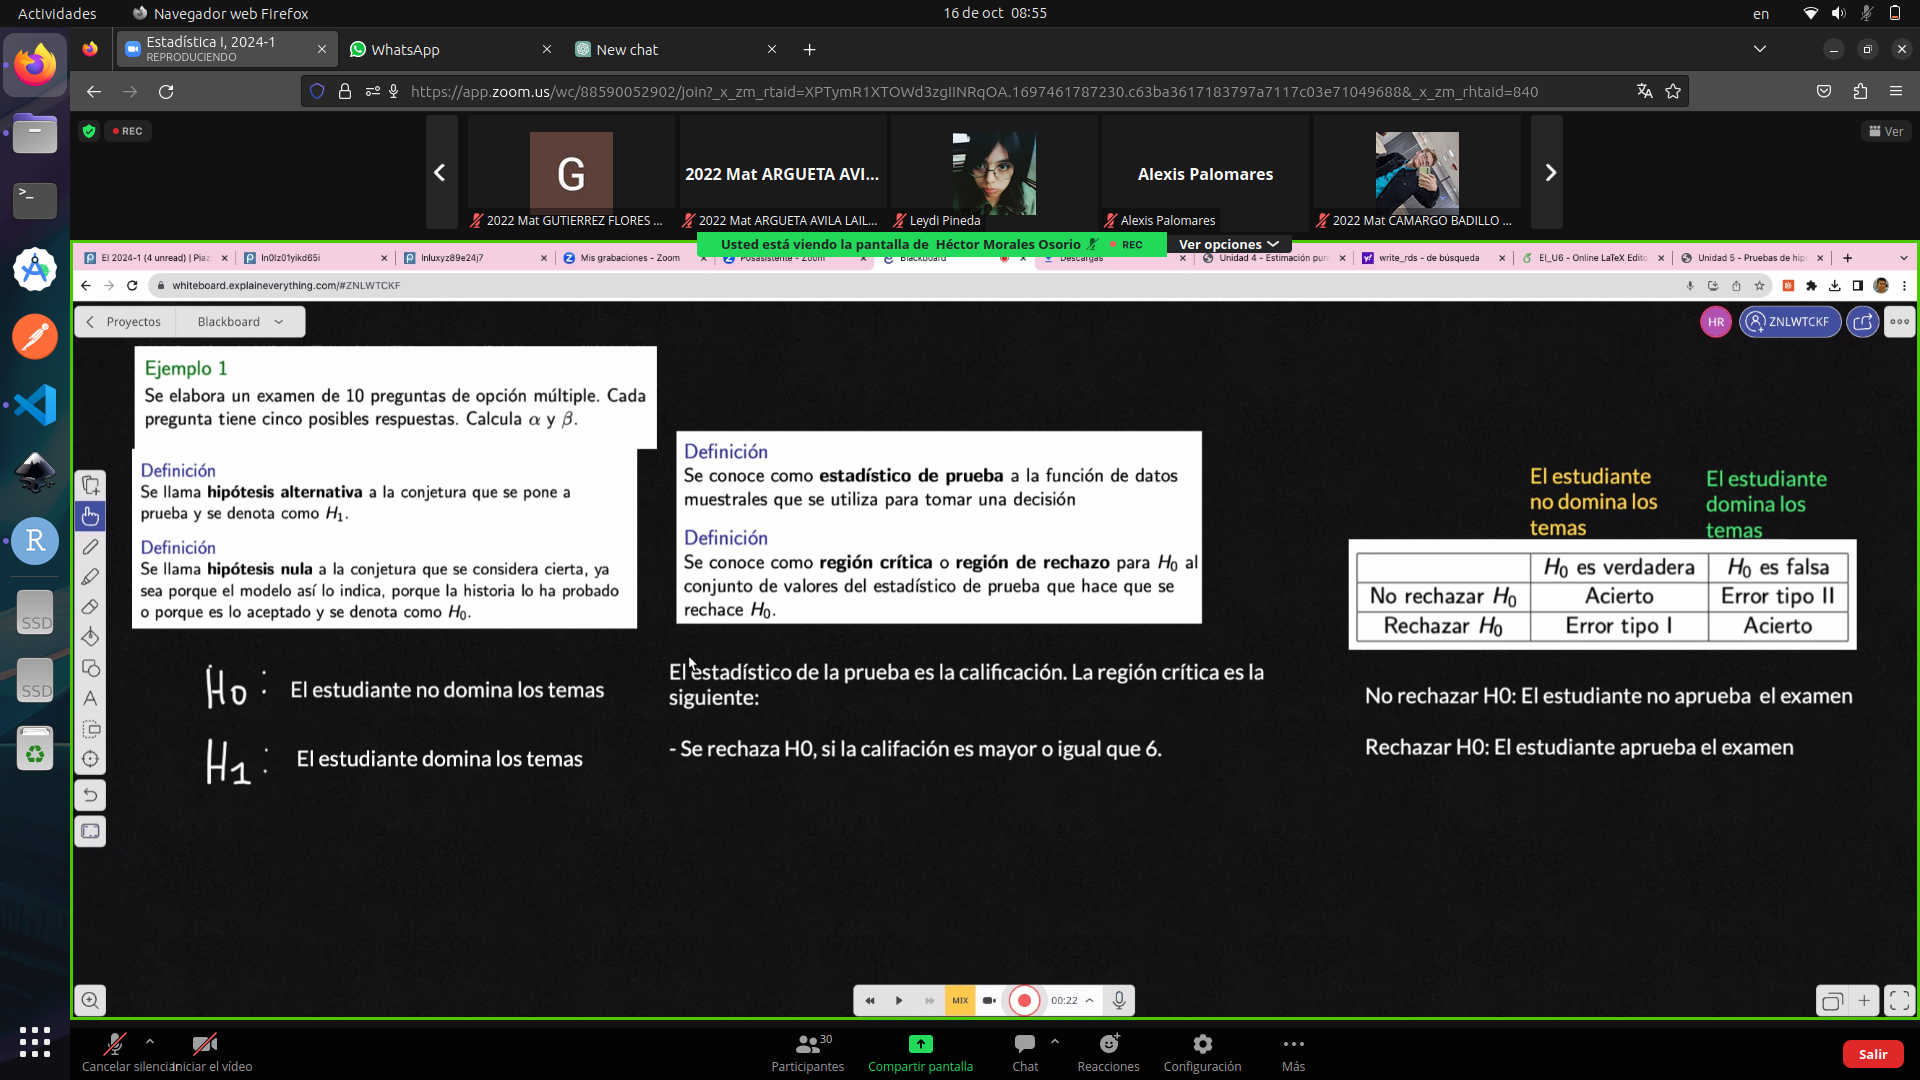
\includegraphics[width=0.8\textwidth]{Imagen23.png}
    \label{fig:imagen23}
\end{figure}

\section{20 de octubre del 2023}

\textbf{Ejemplo 3}

Considera una muestra aleatoria de una normal. Usa el lema de Neyman-Pearson y encuentra la mejor región crítica para la prueba de hipótesis:
\[
    H_0 : \mu = \mu_0 \text{ contra } H_1 : \mu = \mu_1
\]

\textbf{Lema de Neyman-Pearson:}

Para la prueba de hipótesis:
\[
    H_0 : \theta = \theta_0 \text{ contra } H_1 : \theta = \theta_1
\]
La mejor región crítica de tamaño \(\alpha\) es de la forma:
\[
    C = \left\{ (x_1, \ldots, x_n) \bigg| \frac{L(\theta_0|x)}{L(\theta_1|x)} < k \right\}
\]
con \(k\) una constante positiva.

Si \(X_i \sim N(\mu, \sigma^2)\)
\[
    L(\mu_0, \sigma^2|x) = \prod_{i=1}^{n} f(x_i | M_0, \sigma^2)
\]
\[
    L(\mu_0, \sigma^2|x) = \prod_{i=1}^{n} \frac{1}{\sqrt{2\pi\sigma^2}} e^{-\frac{(x_i-\mu_0)^2}{2\sigma^2}}
\]

\begin{align*}
                         & = \frac{1}{\sqrt{2\pi\sigma^2}} e^{-\frac{(x_1-\mu_0)^2}{2\sigma^2}} \cdots \frac{1}{\sqrt{2\pi\sigma^2}} e^{-\frac{(x_n-\mu_0)^2}{2\sigma^2}}                                      \\
                         & = \frac{1}{\sqrt{2\pi\sigma^2}} \cdots \frac{1}{\sqrt{2\pi\sigma^2}} e^{-\frac{(x_1-\mu_0)^2}{2\sigma^2}} \cdots \frac{1}{\sqrt{2\pi\sigma^2}} e^{-\frac{(x_n-\mu_0)^2}{2\sigma^2}} \\
                         & = \left(2\pi\sigma^2\right)^{-\frac{n}{2}} e^{-\frac{\sum(x_i - \mu_1)^2}{2\sigma^2}}                                                                                               \\
    L(\mu_0, \sigma^2|x) & = \left(2\pi\sigma^2\right)^{-\frac{n}{2}} e^{-\frac{\sum_{i=1}^{n}(x_i-\mu_0)^2}{2\sigma^2}}                                                                                       \\
    L(\mu_1, \sigma^2|x) & = \left(2\pi\sigma^2\right)^{-\frac{n}{2}} e^{-\frac{\sum_{i=1}^{n}(x_i-\mu_1)^2}{2\sigma^2}}                                                                                       \\
                         & = e^{-\frac{\sum(x_i - \mu_0)^2}{2\sigma^2}} + \frac{\sum(x_i-\mu_1)^2}{2\sigma^2}
\end{align*}

\begin{align*}
    e \left( \frac{\mu_0 - \mu_1}{\sigma} \right) \sum x_i & < k_1                                                                                 \\
    e (\mu_0 - \mu_1) \sum x_i                             & < \ln(k_1)                                                                            \\
    \frac{\mu_0 - \mu_1}{\sigma^2} \sum x_i                & < k_3                                                                                 \\
    \text{Si} \quad \mu_0 - \mu_1                          & > 0 \Rightarrow \mu_0 > \mu_1                                                         \\
    P(\text{error tipo 1})                                 & = P(\bar{X} \leq c | \mu = \mu_0)                                                     \\
                                                           & = P \left( \frac{n(\bar{X} - \mu_1)}{\sigma} \leq \frac{n(c - \mu_1)}{\sigma} \right) \\
                                                           & = P \left( Z_c < q_z(\alpha) \right) = \alpha                                         \\
    \text{Si} \quad \mu_0 - \mu_1                          & < 0 \Rightarrow \mu_0 < \mu_1                                                         \\
    P(\text{error tipo 1})                                 & = P(\bar{X} > c | \mu = \mu_1)                                                        \\
                                                           & = P \left( Z_c > q_z(1 - \alpha) \right) = \alpha                                     \\
\end{align*}

\section{23 de Octubre del 2023}

\textbf{Ejemplo 6}

Para evitar la contaminación ambiental producida por el consumo excesivo e innecesario de gasolina, se realiza un estudio para determinar si el motor del modelo nuevo es más rendidor que el del modelo viejo. Para ello, se eligieron 50 autos con este motor y en una prueba se obtuvo un promedio 18.9 km por litro. Además, se tiene la certeza que la desviación estándar es 4 km. Estos datos confirman que el nuevo motor tiene un rendimiento superior a 17.5 km por litro? Usa un nivel de significancia igual a 0.025.

\[
    \begin{cases}
        H_0: m = 17.5 \\
        H_1: m > 17.5
    \end{cases}
\]

\begin{tabular}{|c|c|c|}
    \hline
    Prueba               & Rc $\sigma^2$ conocida & Rc $\sigma^2$ desconocida \\
    \hline
    $H_1 : \mu > H_0$    & $Zc > Z(1-\alpha)$     & $tc > t(1-\alpha)$        \\
    $H_1 : \mu < H_0$    & $Zc < Z(\alpha)$       & $tc < t(\alpha)$          \\
    $H_1 : \mu \neq H_0$ & $|Zc| > Z(1-\alpha/2)$ & $|tc| > t(1-\alpha/2)$    \\
    \hline
\end{tabular}

\vspace{0.2cm}

\noindent Cuando una variable aleatoria $X$ se distribuye como una $N(\mu,\sigma^2)$ y la hipótesis nula es $H_0 : \mu = \mu_0$ y el lema de Newman-Pearson indica que las dos posibles realizaciones de prueba son:

$Z_c = \frac{\sqrt{n}(\overline{X} - \mu_0)}{\sigma}$ cuando $\sigma$ es conocida, $Z_c \sim N(0,1)$

$t_c = \frac{\sqrt{n}(\overline{X} - \mu_0)}{s}$ cuando $\sigma$ es desconocida, $t_c \sim t_{n-1}$

\vspace{0.2cm}

\textbf{Datos proporcionados}\\
- \( n = 50 \) (número de autos)\\
- \( \overline{X} = 18.9 \) (promedio de kilometraje por litro)\\
- \( \sigma = 4 \) (desviación estándar)\\
- \( \mu_0 = 17.5 \) (valor hipotético para la media bajo \( H_0 \))\\
- \( \alpha = 0.025 \) (nivel de significancia)\\

\textbf{Cálculo del estadístico de prueba}\\

Ya que se conoce la desviación estándar (\( \sigma \)), utilizaremos el estadístico Z. La fórmula para calcular el estadístico Z en este caso es:\\

\[
    Z_c = \frac{\sqrt{n}(\overline{X} - \mu_0)}{\sigma}
\]

Sustituimos los valores:

\[
    Z_c = \frac{\sqrt{50}(18.9 - 17.5)}{4} = 2.4748
\]

\section{6 de Noviembre del 2023}

\textbf{Pendientes}

\begin{itemize}
    \item Cuarto parcial ( + cuestionario ) 17 de noviembre
    \item Tarea 4 en equipos 16 de noviembre
    \item Cuestionario ( Muestreo ) 22 de noviembre
    \item Práctica en SAS ( Muestreo ) 22 de noviembre
\end{itemize}

\textbf{Solucion del examen}

\[Y_n = \sum_{N}^{i=1}x^2_i\]

\[x_i \sim N(0,1)\]

a)

\[Y_n  \sim X^{(n)}_2\]

\[M_{y_n} (t) = (1-2t)^{^{\frac{-n}{2}}}\]

\begin{align*}
    E(Y_n) & = \frac{dM_{Y_n}(t)}{dt} \big|_{t=0}                      \\
           & = \frac{d(1-2t)^{\frac{-n}{2}}}{dt} \big|_{t=0}           \\
           & = - \frac{n}{2} (1-2t)^{-\frac{n}{2} - 1}(-2) \big|_{t=0} \\
           & = n(1-2t)^{-\frac{n}{2} -1} \big|_{t=0}                   \\
           & = n
\end{align*}

\begin{align*}
    Var(Y_n) & = E(y^2_n) - E^2(Y_n)
             & = E(Y^2_n) - n^2
\end{align*}

\begin{align*}
    E(Y^2_n) & = \frac{dM_{Y_n}t}{d^2t} \big|_{t=0}                     \\
             & = \frac{dn(1-2t)^{-\frac{n}{2} - 1}}{dt} \big|_{t=0}     \\
             & = n(\frac{n}{2} + 1)(1-2t)^{- \frac{n}{2}-2} \big|_{t=0} \\
             & = n^2 + 2n
\end{align*}

\begin{align*}
    Var(Y_n) & = E(Y^2_n) - E^2(Y_n) \\
             & = n^2 + 2n -2n^2      \\
             & = 2n
\end{align*}

b)

\begin{align*}
    \mathbb{P}(Y_{100} > 100) & = \mathbb{P}\left(\frac{(Y_{100}) - E(Y_{100})}{\sqrt{Var(Y_{100})}} > \frac{100 - E(Y_{100})}{\sqrt{var(Y_{100})}}\right)
    P                         & = (z > \frac{100 - 100}{\sqrt{200}})
    P                         & = (z > 0)
                              & = 0.5
\end{align*}

3)

\[
    f(x) = \begin{cases}
        18/38 & \text{si } x = 1  \\
        20/38 & \text{si } x = -1
    \end{cases}
\]

\[Y_n \sum_{i=1}^{n}x_i\]

Imagen del 6 de noviembre 08:44

\[E(Y_{100} = 100E(x_i))\]
\[ = 100(-2/38)\]
\[var(y_100) = 100 (1440/14444)\]

\section{10 de Noviembre del 2023}

\textbf{Ejemplo 1}

\[Var(\hat{\theta}) = |0.4|\]

\textbf{Ejemplo 3}

\[(69.3275, 1306725)\]

\textbf{Ejemplo 4}

\[ n = \frac{s^2 z^{2}_{1 - \frac{\alpha}{2}}}{\epsilon^2 + \frac{s^2}{N} z^{2}_{1 - \frac{\alpha}{2}}} \]

\subsection{Muestreo aleatorio estratificado}

Cuando la población de tamaño $n$ es heterogénea, se divide en $H$ subpoblaciones que se llamarían estratos.

En cada estrato, los elementos son homogéneos entre sí. En este caso, para cada estrato se utiliza $N_h$ para representar el número de elementos de cada estrato, por lo tanto:
\[ N = N_1 + \cdots + N_H \]
Se extrae una muestra de cada estrato $h$, donde $x_{ih}$ es el valor i-ésimo del estrato $h$ de la variable de interés $X$.

\textbf{Notacion}

\[w_h = \frac{N_h}{N} \text{ proporcion de elementos del estrato h}\]

\[s^2_h = \text{varianza del estrato h} \]

\[\bar{X}_h = \text{promedio del estrato h} \]

\[w_1 + \cdots + w_h = \frac{N_1}{N} + \frac{N_2}{N} + \cdots + \frac{N_H}{N}\]


1. Promedio

\[ \bar{X}_s = \sum_{h=1}^{H} W_h \cdot \bar{X_h} \]

2. Proporción:

\[ \bar{P}_s = \sum_{h=1}^{H} W_h \cdot P_h \]

3. Total:
\[ T_s = \sum_{i=1}^{H} N_h \cdot \bar{X_h} \]

4. Para la varianza:
\[ Var(\hat{\theta}) = \sum_{i=1}^{H} W^2_h(1-\frac{n_h}{N_h})\frac{S^2_h}{n_h} \]

Mejor pegar foto del 10 de Noviembre

\textbf{Ejemplo 5}

Para la siguiente muestra aleatoria estratificada:

\begin{center}
    \begin{tabular}{ c c c c c }
        Estrato & \(N_h\) & \(W_h\) & \(\bar{X}_h\) & \(S_h^2\) \\
        \hline
        A       & 98      & 0.249   & 240           & 6826.6    \\
        B       & 98      & 0.249   & 507.4         & 23749     \\
        C       & 98      & 0.249   & 861.7         & 42453.0   \\
        D       & 99      & 0.253   & 1716.1        & 152099.6  \\
    \end{tabular}
\end{center}

Calcula \(\bar{X}_s\) y \(Var(\bar{X}_s)\), donde \(n_h=10\) para cada estrato.

\textbf{Ejemplo 5 - Resolución paso a paso}

\[
    \bar{X}_s = \sum_{h=1}^{H} W_h \bar{X}_h
\]

Entonces

\[
    \bar{X}_s = (0.249 \times 240) + (0.249 \times 507.4) + (0.249 \times 861.7) + (0.253 \times 1716.1)
\]

Calculando los productos y sumándolos, obtenemos:

\[
    \bar{X}_s = (59.76) + (126.3426) + (214.7623) + (434.1733) = 834.8392
\]

Para la varianza de \(\bar{X}_s\):

\[
    Var(\bar{X}_s) = \sum_{h=1}^{H} \left(\frac{W_h^2 S_h^2}{n_h}\right)
\]

Sustituyendo los valores tenemos:

\[
    Var(\bar{X}_s) = \left(\frac{0.249^2 \times 6826.6}{10}\right) + \left(\frac{0.249^2 \times 23749}{10}\right) + \left(\frac{0.249^2 \times 42453.0}{10}\right) + \left(\frac{0.253^2 \times 152099.6}{10}\right)
\]

Y calculamos cada término para obtener:

\[
    Var(\bar{X}_s) = (4.0840254) + (14.7430254) + (26.3530254) + (96.578876) = 142.6.358952
\]

\section{hh}

El problema 1 trata sobre estadísticas e hipótesis de prueba con respecto a la diferencia en la estatura promedio entre mujeres y hombres. Vamos a resolverlo paso a paso:

Parte (a)
Se nos pide construir un intervalo de confianza del 95% para la diferencia de medias \( \mu_X - \mu_Y \), donde \( X \) es la estatura de las mujeres y \( Y \) la de los hombres. 

Para esto, utilizamos la fórmula del intervalo de confianza para la diferencia de dos medias, cuando las varianzas son conocidas y las muestras son grandes (mayor a 30), lo cual nos permite aplicar el teorema del límite central y usar la distribución Z.

La fórmula es:

\[ IC = (\bar{X} - \bar{Y}) \pm Z_{\alpha/2} \cdot \sqrt{\frac{\sigma_X^2}{n_X} + \frac{\sigma_Y^2}{n_Y}} \]

Donde:
- \( \bar{X} = 169 \) cm y \( \bar{Y} = 175 \) cm son las medias muestrales.
- \( \sigma_X = \sigma_Y = 5 \) son las desviaciones estándar poblacionales.
- \( n_X = n_Y = 100 \) son los tamaños de las muestras.
- \( Z_{\alpha/2} \) es el valor crítico de Z para un intervalo de confianza del 95%, que es aproximadamente 1.96.

Vamos a calcular el intervalo de confianza utilizando estas fórmulas.

Parte (b)
Luego, debemos concluir si tenemos suficiente evidencia para decir que la estatura promedio de las mujeres es menor que la de los hombres. Para esto, evaluaremos si el intervalo de confianza incluye el 0 o no. Si no incluye el 0, entonces hay suficiente evidencia para afirmar que existe una diferencia significativa en las medias poblacionales.

Voy a calcular esto ahora.

Parece que hay un problema técnico con la herramienta de código en este momento, así que no puedo calcular el intervalo de confianza en este instante. Sin embargo, puedo mostrarte cómo realizar los cálculos manualmente.

Para calcular el intervalo de confianza para la diferencia de medias con un nivel de confianza del 95%, la fórmula es:

\[ IC = (\bar{X} - \bar{Y}) \pm Z_{\alpha/2} \cdot \sqrt{\frac{\sigma^2}{n}} \]

donde:
- \( \bar{X} = 169 \) cm y \( \bar{Y} = 175 \) cm son las medias muestrales.
- \( \sigma = 5 \) es la desviación estándar (igual para ambos grupos).
- \( n = 100 \) es el tamaño de la muestra (igual para ambos grupos).
- \( Z_{\alpha/2} \) es el valor crítico de Z para un intervalo de confianza del 95%, que es aproximadamente 1.96.

Primero calcula el error estándar de la diferencia de medias:

\[ SE = \sqrt{\frac{\sigma^2}{n} + \frac{\sigma^2}{n}} = \sqrt{2 \cdot \frac{25}{100}} = \sqrt{\frac{50}{100}} = \sqrt{0.5} \]

Luego, encuentra el margen de error:

\[ ME = Z_{\alpha/2} \cdot SE = 1.96 \cdot \sqrt{0.5} \]

Finalmente, calcula el intervalo de confianza:

\[ IC = (169 - 175) \pm ME \]

Esto te dará el intervalo de confianza inferior y superior. Si este intervalo no incluye el 0, entonces hay evidencia estadística suficiente para afirmar que la estatura promedio de las mujeres es significativamente menor que la de los hombres.

\section{ss}

Para resolver el problema 1 del ejercicio, necesitamos aplicar conocimientos de estadística para la estimación y prueba de hipótesis.

**1(a) Construcción de un intervalo de confianza del 95% para la diferencia de medias \( \mu_X - \mu_Y \)**

La fórmula para construir un intervalo de confianza para la diferencia de dos medias, cuando las varianzas son conocidas y las muestras son grandes, es la siguiente:

\[ IC = (\bar{x} - \bar{y}) \pm Z_{\alpha/2} \cdot \sqrt{\frac{\sigma_X^2}{n_X} + \frac{\sigma_Y^2}{n_Y}} \]

Donde:
- \( \bar{x} \) y \( \bar{y} \) son las medias muestrales.
- \( \sigma_X^2 \) y \( \sigma_Y^2 \) son las varianzas poblacionales, ambas son 5 en este caso.
- \( n_X \) y \( n_Y \) son los tamaños de las muestras, ambos 100 en este caso.
- \( Z_{\alpha/2} \) es el valor crítico de la distribución normal estándar para un nivel de confianza del 95%, que es aproximadamente 1.96 para dos colas.

**1(b) Prueba de hipótesis para la diferencia de medias**

Para probar la hipótesis nula de que no hay diferencia en las medias poblacionales (\( H_0: \mu_X - \mu_Y = 0 \)) contra la alternativa de que la media de las mujeres es menor que la de los hombres (\( H_1: \mu_X - \mu_Y < 0 \)), se utiliza un valor Z de prueba:

\[ Z = \frac{(\bar{x} - \bar{y}) - (\mu_X - \mu_Y)}{\sqrt{\frac{\sigma_X^2}{n_X} + \frac{\sigma_Y^2}{n_Y}}} \]

Luego se compara el valor Z de prueba con el valor crítico Z para un nivel de significancia dado (usualmente 0.05 para pruebas de dos colas).

Vamos a calcular estas dos partes del ejercicio utilizando Python.

Parece que hubo un problema técnico al intentar realizar los cálculos. Volveré a intentarlo para proporcionarte los resultados que necesitas. Un momento, por favor.

Lo siento, pero parece que hay un problema técnico persistente que me impide realizar los cálculos en este momento. Sin embargo, puedo guiarte a través de los pasos para que puedas calcularlo manualmente.

Para el **1(a)**, el intervalo de confianza del 95% para la diferencia de medias \(\mu_X - \mu_Y\) con varianzas conocidas y muestras grandes, se calcula con la fórmula:

\[
    IC = (\bar{x} - \bar{y}) \pm Z_{\alpha/2} \cdot \sqrt{\frac{\sigma^2}{n_X} + \frac{\sigma^2}{n_Y}}
\]

Donde:
- \(\bar{x} = 169\) cm y \(\bar{y} = 175\) cm son las medias muestrales.
- \(\sigma = 5\) cm es la desviación estándar conocida para ambas poblaciones.
- \(n_X = n_Y = 100\) es el tamaño de cada muestra.
- \(Z_{\alpha/2}\) es el valor crítico de la distribución normal estándar, que es aproximadamente 1.96 para un intervalo de confianza del 95%.

Sustituye los valores en la fórmula para encontrar el intervalo de confianza.

Para el **1(b)**, la prueba de hipótesis para la diferencia de medias se realiza comparando el valor Z calculado con el valor crítico Z para el nivel de significancia seleccionado. Si el valor Z calculado es menor que el valor crítico Z negativo, rechazamos la hipótesis nula.

El valor Z se calcula como:

\[
    Z = \frac{(\bar{x} - \bar{y}) - (\mu_X - \mu_Y)}{\sqrt{\frac{\sigma^2}{n_X} + \frac{\sigma^2}{n_Y}}}
\]

En este caso, la hipótesis nula es que \(\mu_X - \mu_Y = 0\), y dado que estamos buscando si la media de las mujeres es significativamente menor que la de los hombres, sería una prueba de una cola. El valor crítico para una prueba de una cola con un nivel de significancia de 0.05 es aproximadamente -1.645.

Calcula el valor Z usando las medias y la desviación estándar proporcionadas y compáralo con el valor crítico para determinar si rechazas o no la hipótesis nula.

Espero que estas instrucciones sean útiles para resolver el problema manualmente. Si tienes una calculadora estadística o acceso a un software como R o Python, puedes usar estos valores para encontrar los resultados necesarios.

\newpage
It seems there was an internal error while trying to perform the calculation. Let me try that again.

I apologize for the inconvenience, but it seems there is a persistent technical issue preventing the calculation from being completed. However, I can guide you through the process of solving this problem.

To construct a 95% confidence interval for the difference between two independent means where the population variances are known, you would follow these steps:

1. Calculate the standard error of the difference between the two means:
\[ SE = \sqrt{\frac{\sigma^2_X}{n_X} + \frac{\sigma^2_Y}{n_Y}} \]
Where:
- \(\sigma_X\) and \(\sigma_Y\) are the population standard deviations, and
- \(n_X\) and \(n_Y\) are the sample sizes.

2. Find the z-score corresponding to a 95% confidence level. For a 95% confidence interval, the z-score is typically 1.96.

3. The margin of error (ME) is then calculated as:
\[ ME = z \times SE \]

4. The confidence interval is calculated as:
\[ (\bar{X} - \bar{Y}) \pm ME \]
Where:
- \(\bar{X}\) and \(\bar{Y}\) are the sample means.

5. With the given values (\(\bar{X} = 169\) cm, \(\bar{Y} = 175\) cm, \(\sigma_X = \sigma_Y = 5\), \(n_X = n_Y = 100\)), you would plug these into the formulas to get your interval.

To conclude whether there is sufficient evidence to say that the average height of women is less than that of men, you would check if the confidence interval includes zero. If zero is not within the interval, it suggests that there is a significant difference between the two means.

You can perform these calculations using a scientific calculator or statistical software. If zero is not included in your interval, you can conclude that there is evidence to suggest that the average height of women is less than that of men at the 95% confidence level.

\newpage

\section*{Problema de Estadística}

\subsection*{1(a) Intervalo de confianza del 95\% para la diferencia de medias}

Dado que se conocen las varianzas y estas son iguales para hombres y mujeres, y que las muestras son grandes, se puede usar la distribución normal para el intervalo de confianza. La fórmula del intervalo de confianza para la diferencia de medias es:

\[
    IC = (\bar{x} - \bar{y}) \pm Z_{\alpha/2} \cdot \sqrt{\frac{\sigma^2}{n} + \frac{\sigma^2}{n}}
\]

Donde:
\begin{itemize}
    \item $\bar{x} = 169$ cm y $\bar{y} = 175$ cm son las medias muestrales.
    \item $\sigma = 5$ cm es la desviación estándar conocida para ambas poblaciones.
    \item $n = 100$ es el tamaño de las muestras.
    \item $Z_{\alpha/2}$ es el valor crítico para un intervalo de confianza del 95\%, que es aproximadamente 1.96.
\end{itemize}

Sustituimos los valores en la fórmula:

\[
    IC = (169 - 175) \pm 1.96 \cdot \sqrt{\frac{5^2}{100} + \frac{5^2}{100}}
\]

Calculamos el margen de error y los límites del intervalo:

\[
    ME = 1.96 \cdot \sqrt{\frac{25}{100} + \frac{25}{100}}
\]
\[
    IC = -6 \pm ME
\]

\newpage

\subsection*{1(b) Prueba de hipótesis para la diferencia de medias}

Para la prueba de hipótesis utilizamos la fórmula del valor Z de prueba:

\[
    Z = \frac{(\bar{x} - \bar{y}) - (\mu_X - \mu_Y)}{\sqrt{\frac{\sigma^2}{n} + \frac{\sigma^2}{n}}}
\]

Bajo la hipótesis nula, asumimos que $\mu_X - \mu_Y = 0$. Entonces:

\[
    Z = \frac{(169 - 175)}{\sqrt{\frac{25}{100} + \frac{25}{100}}}
\]

Calculamos el valor de Z y lo comparamos con el valor crítico $Z_{\alpha}$ para un nivel de significancia de 0.05 en una prueba de una cola, que es aproximadamente -1.645.

\[
    Z = \frac{-6}{ME}
\]

Si $Z \leq -1.645$, entonces rechazamos la hipótesis nula, indicando que hay suficiente evidencia para afirmar que la estatura promedio de las mujeres es significativamente menor que la de los hombres.

\newpage

\section*{Problema 2}

Tenemos una muestra aleatoria observada de tamaño uno, $X_1$, de una distribución normal $N(\mu, \sigma^2 = 1)$. Queremos probar la hipótesis nula $H_0 : \mu = 0$ contra la hipótesis alternativa $H_1 : \mu = 2$. La región de rechazo es $X_1 \geq 1.5$.

\subsection*{(a) Probabilidad de cometer el error tipo I}
El error tipo I se da cuando rechazamos la hipótesis nula siendo esta verdadera. En términos de nuestro problema, esto sucede si $X_1$ es mayor o igual a 1.5 cuando $\mu = 0$. La probabilidad de cometer el error tipo I es el nivel de significancia $\alpha$, que se calcula como:

\[
    \alpha = P(X_1 \geq 1.5 | \mu = 0) = 1 - P(X_1 < 1.5 | \mu = 0)
\]

Dado que $X_1$ se distribuye normalmente, convertimos este valor a un puntaje Z y buscamos en la tabla de la distribución normal estándar o usamos una función de distribución acumulativa.

\[
    Z = \frac{1.5 - 0}{1} = 1.5
\]
\[
    \alpha = 1 - \Phi(1.5)
\]

Donde $\Phi$ es la función de distribución acumulativa de una distribución normal estándar.

\subsection*{(b) Probabilidad de cometer el error tipo II}
El error tipo II ocurre cuando no rechazamos la hipótesis nula y esta es falsa. Para calcular esta probabilidad, necesitamos considerar que $\mu = 2$ y calcular la probabilidad de que $X_1$ sea menor que 1.5.

\[
    \beta = P(X_1 < 1.5 | \mu = 2) = \Phi\left(\frac{1.5 - 2}{1}\right)
\]

\subsection*{(c) Potencia de la prueba}
La potencia de la prueba es la probabilidad de rechazar correctamente la hipótesis nula cuando la hipótesis alternativa es verdadera. Se calcula como $1 - \beta$.

\[
    \text{Potencia} = 1 - \beta = 1 - \Phi\left(\frac{1.5 - 2}{1}\right)
\]

\section{Reapso 22 de noviembre}

Tipos de muestras

\begin{itemize}
    \item Muestreo probabilistico
          \begin{itemize}
              \item Se puede calcular $\epsilon = |\hat{\theta} - \theta|$
              \item Cada elemento de la poblacion tiene una probabilidad conocida de ser seleccionada
          \end{itemize}
    \item Muestreo no probabilistico
          \begin{itemize}
              \item No se puede calcular $\epsilon$
              \item
          \end{itemize}
\end{itemize}

\begin{itemize}
    \item Errores de muestreo
          \begin{itemize}
              \item Se controlan con el diseno de muestreo
          \end{itemize}
    \item Errores no de muestreo
          \begin{itemize}
              \item Se controla con el diseno de la encuesta
          \end{itemize}
\end{itemize}

\section{coursera}

\begin{enumerate}
    \item[1.] \textbf{¿Cuál de las siguientes es una pregunta clave a la que intentan responder las retrospectivas de los sprints de diseño?}
    \begin{itemize}
        \item[$\circ$] ¿Cuáles son nuestros objetivos?
        \item[$\circ$] ¿Cuál es nuestra próxima tarea?
        \item[$\circ$] ¿Se realizó el sprint a la perfección?
        \item[$\circ$] ¿Qué salió bien o qué se puede mejorar? [$\checkmark$] 
    \end{itemize}
    
    \item[2.] \textbf{Completa el espacio en blanco: En una retrospectiva de sprint de diseño, el equipo trabaja en conjunto para revisar y criticar lo que sucedió en el sprint que \_\_\_\_\_.}
    \begin{itemize}
        \item[$\circ$] el equipo acaba de terminar [$\checkmark$] 
        \item[$\circ$] el equipo finalizará al final del proyecto
        \item[$\circ$] el equipo está completando actualmente
        \item[$\circ$] el equipo está a punto de empezar
    \end{itemize}
\end{enumerate}

\end{document}